\documentclass{article}

% if you need to pass options to natbib, use, e.g.:
%     \PassOptionsToPackage{numbers, compress}{natbib}
% before loading neurips_2020

% ready for submission
% \usepackage{neurips_2020}

% to compile a preprint version, e.g., for submission to arXiv, add add the
% [preprint] option:
%     \usepackage[preprint]{neurips_2020}

% to compile a camera-ready version, add the [final] option, e.g.:
%     \usepackage[final]{neurips_2020}

% to avoid loading the natbib package, add option nonatbib:
\usepackage[nonatbib, preprint]{neurips_2020}

\usepackage[utf8]{inputenc} % allow utf-8 input
\usepackage[T1]{fontenc}    % use 8-bit T1 fonts
\usepackage{hyperref}       % hyperlinks
\usepackage{url}            % simple URL typesetting
\usepackage{booktabs}       % professional-quality tables
\usepackage{amsfonts}       % blackboard math symbols
\usepackage{nicefrac}       % compact symbols for 1/2, etc.
\usepackage{microtype}      % microtypography
\usepackage{graphicx}
\usepackage{enumitem}
\usepackage{amsmath}
\usepackage{esvect}
\usepackage{xcolor}
\usepackage{enumitem}
\usepackage{siunitx}
\usepackage{mathtools}
\usepackage{caption}
\usepackage{diagbox}
\usepackage{multirow}
\usepackage{float}
\usepackage{diagbox}
\usepackage{multirow}
\usepackage{xspace}
\usepackage[title]{appendix}

\setlist{noitemsep}


% \let\oldsection\section
% \renewcommand\section{\clearpage\oldsection}


\long\def\comment#1{}

\newcommand{\varbold}[1]{\textcolor{black}{#1}}

% \newcommand{\niv}[1]{\comment{#1\}}}
% \newcommand{\assaf}[1]{\comment{#1\}}}
% \newcommand{\ben}[1]{\comment{#1\}}}
% \newcommand{\michal}[1]{\comment{#1\}}}
% \newcommand{\niv}[1]{\textcolor{orange}{#1}}
% \newcommand{\assaf}[1]{\textcolor{cyan}{#1}}
% \newcommand{\ben}[1]{\textcolor{purple}{#1}}
% \newcommand{\michal}[1]{\textcolor{red}{#1}}

\newcommand{\niv}[1]{\textcolor{black}{#1}}
\newcommand{\assaf}[1]{\textcolor{black}{#1}}
\newcommand{\ben}[1]{\textcolor{black}{#1}}
\newcommand{\michal}[1]{\textcolor{black}{#1}}


\newcommand{\nivc}[1]{\comment{#1\}}}
\newcommand{\assafc}[1]{\comment{#1\}}}
\newcommand{\benc}[1]{\comment{#1\}}}
\newcommand{\michalc}[1]{\comment{#1\}}}
% \newcommand{\nivc}[1]{\textcolor{orange}{\{Niv: #1\}}}
% \newcommand{\assafc}[1]{\textcolor{cyan}{\{Assaf: #1\}}}
% \newcommand{\benc}[1]{\textcolor{purple}{\{Ben: #1\}}}
% \newcommand{\michalc}[1]{\textcolor{red}{\{Michal: #1\}}}

\newcommand{\CC}{\textsc{CC}\xspace}

\usepackage{biblatex}
% \renewcommand{\bibname}{main.bib}
\addbibresource{main.bib}
% \bibliography{main.bib}
\vspace{-0.4cm}

\title{From Discrete to Continuous Convolution Layers}
\begin{document}
\author{Assaf Shocher\thanks{equal contribution}
\qquad Ben Feinstein\footnotemark[1]
\qquad Niv Haim\footnotemark[1]
\qquad Michal Irani\\
\small 
Dept. of Computer Science and Applied Math, The Weizmann Institute of Science
}

\maketitle
 
\begin{abstract}
Grokking, or sudden generalization that occurs after prolonged overfitting, is a surprising phenomenon that has challenged our understanding of deep learning. While a lot of progress has been made in understanding grokking, it is still not clear why generalization is delayed and why grokking often does not happen without regularization. In this work we argue that without regularization, grokking tasks push models to the edge of numerical stability, introducing floating point errors in the Softmax that we refer to as \emph{Softmax Collapse} (SC). We show that SC prevents grokking and that mitigating SC leads to grokking \textit{without} regularization. Investigating the root cause of SC, we find that beyond the point of overfitting, the gradients strongly align with what we call the \emph{naïve loss minimization} (NLM) direction. This component of the gradient does not change the predictions of the model but decreases the loss by scaling the logits, usually through the scaling of the weights along their current direction. We show that this scaling of the logits explains the delay in generalization characteristic of grokking, and eventually leads to SC, stopping learning altogether. To validate these hypotheses, we introduce two key contributions that mitigate the issues faced in grokking tasks: (i) $\stablemax$, a new activation function that prevents SC and enables grokking without regularization, and (ii) $\ograd$, a training algorithm that leads to quick generalization in grokking tasks by preventing NLM altogether. These contributions provide new insights into grokking, shedding light on its delayed generalization, reliance on regularization, and the effectiveness of known grokking-inducing methods. Code for this paper can be found at: \url{https://github.com/LucasPrietoAl/grokking-at-the-edge-of-numerical-stability}.

\end{abstract}




\section{Introduction}


Deep learning has been transformative for a variety of fields such as natural language processing~\citep{devlin2018bert}, computer vision~\citep{krizhevsky2012imagenet}, geometry processing~\citep{qi2017pointnet}, and 3D vision~\citep{deng2018ppfnet}. This rapid proliferation has brought with it surprising phenomena that defy the predictions of classical statistical learning theory.


In this paper we explore one such recently observed phenomenon known as \emph{grokking}, first described by \citet{power2022grokking} as a sudden and unexpected generalization occurring after prolonged overfitting. Although predominantly studied in algorithmic tasks like modular addition or multiplication, recent findings suggest that grokking may be a more pervasive phenomenon, also manifesting in more complex tasks involving vision and language~\citep{lv2024language,humayun2024deep}.


Prior research has consistently observed grokking in settings that involve some form of regularization, such as weight decay~\citep{Barak2022-el, power2022grokking, Nanda2023-hf}. This pattern has motivated investigations into the implicit biases introduced by weight decay, suggesting it may be critical to triggering delayed generalization. For instance, \citet{liu2023omnigrok} argued that weight norms need to be in a narrow range or ``Goldilocks Zone'' for generalization. Similarly, \citet{Varma2023} highlighted weight efficiency of generalizing solutions, and \citet{Nanda2023-hf} argued that weight decay favors simpler, more generalizable solutions. However, recent works have argued that regularization may not be necessary for grokking, at least on shallow networks with Mean Squared Error (MSE) loss \citep{Kumar2023-hz, Lyu2023-ga, Gromov2023-nh}. These works tie grokking to a transition from lazy training \citep{Chizat_Oyallon_Bach_2018} to feature learning. Despite this ongoing work, several aspects in this framing of grokking remain unclear. These include why grokking tasks induce lazy training and why weight decay is often needed to enter the feature learning regime when using deeper models or cross-entropy (CE) loss.


Here we propose a novel account of grokking, outlined in \cref{fig:teaser}, that explains several of the main unanswered questions in the grokking literature. We start by showing that without regularization, grokking is prevented by absorption errors in the \softmax, which we call \emph{Softmax Collapse} (SC). These errors result in zero terms in the gradient and put an end to learning, sometimes before any progress is made in the test performance, resulting in complete overfitting (\cref{fig:teaser}, \textbf{c}). We then argue that SC is caused by what we call \emph{Naïve Loss Minimization} (NLM), as the gradient becomes aligned with a direction that corresponds to scaling up the logits by a constant. While scaling up all the logits does not change the model predictions, it does reduce the CE loss for a network that has reached 100\% training accuracy, with the downside that this eventually leads to numerical errors in \softmax. 
Our findings provide explanations for several key aspects of grokking, including (i) the delayed onset of generalization, (ii) why grokking is often absent without regularization, and (iii) why existing methods designed to induce grokking are effective.

To validate our hypothesis that SC is responsible for the absence of grokking without regularization, we introduce $\bm{\stablemax}$ as a more numerically stable replacement to $\softmax$ in CE loss. This simple change takes models from complete overfitting to grokking (\cref{fig:teaser}, \textbf{c} to \textbf{b}) \textit{without} regularization, in settings where it is normally not observed without it. Similarly, we validate that NLM is responsible for delaying generalization (\cref{fig:teaser}, \textbf{a} to \textbf{b}) and leading to SC by introducing a new optimizer $\ograd$, which only preserves the part of the gradient that is orthogonal to the NLM direction. By doing this, $\ograd$ quickly leads to generalization without the initial overfitting phase that defines grokking (\cref{fig:teaser}, \textbf{b} to \textbf{a}).

Our primary contributions are as follows:
\begin{itemize}[leftmargin=*,topsep=0em,noitemsep]
    \item We observe that cases of overfitting without grokking are due to floating point errors caused by extreme values in the $\softmax$~function, which we term Softmax Collapse (SC;~\cref{sec:floating_points}).
    \item We show that interventions to avoid SC, like greater floating point precision or a new, numerically stable version of Softmax ($\stablemax$), cause grokking in settings where it was previously absent without regularization (\cref{sec:preventing_sc}).
    \item We observe that models move towards SC because overfitting and cross-entropy loss push the model in a direction of uncontrolled logit growth, which we refer to as Naïve Loss Minimization (NLM;~\cref{sec:nlm}).
    \item We demonstrate that NLM can be avoided through a novel optimizer, \ograd, which removes the delay in generalization (\cref{sec:avoiding_nmm}).
\end{itemize}


\begin{figure}[t]
\begin{centering}
    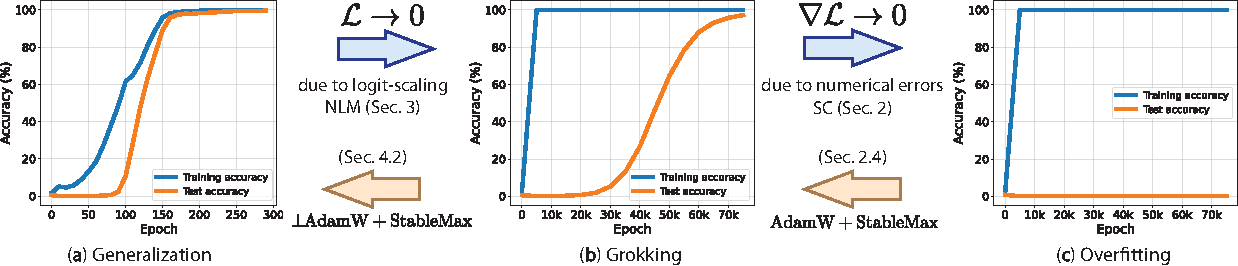
\includegraphics[width=\linewidth]{grokking_iclr_arxiv/figures/grokking.pdf}\vspace{-6mm}
\end{centering}
\caption{Our contributions demonstrated through results obtained in addition modulo 113 task. We show that the delay in generalization induced by NLM can be reversed using the proposed $\perp$\!AdamW ((\textbf{a}) and (\textbf{b})) and that the numerical errors that lead to overfitting instead of grokking can be avoided by using the proposed $\stablemax$ ((\textbf{b}) and (\textbf{c})). \vspace{-5mm}}
\label{fig:teaser}
%\vspace{-3mm}
\end{figure}

\begin{comment}
\begin{figure}[t]
\begin{subfigure}[t]{.32\textwidth}
    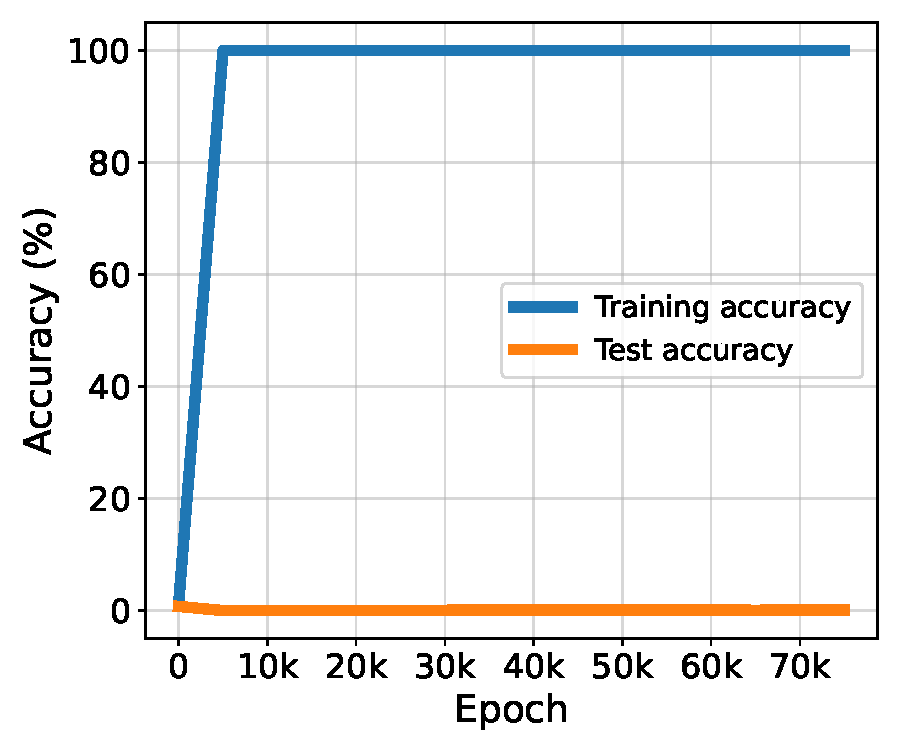
\includegraphics[width=\linewidth]{grokking_iclr/figures/teaser_baseline.pdf}
    \caption{AdamW}
\end{subfigure}
\hfill
\begin{subfigure}[t]{.32\textwidth}
    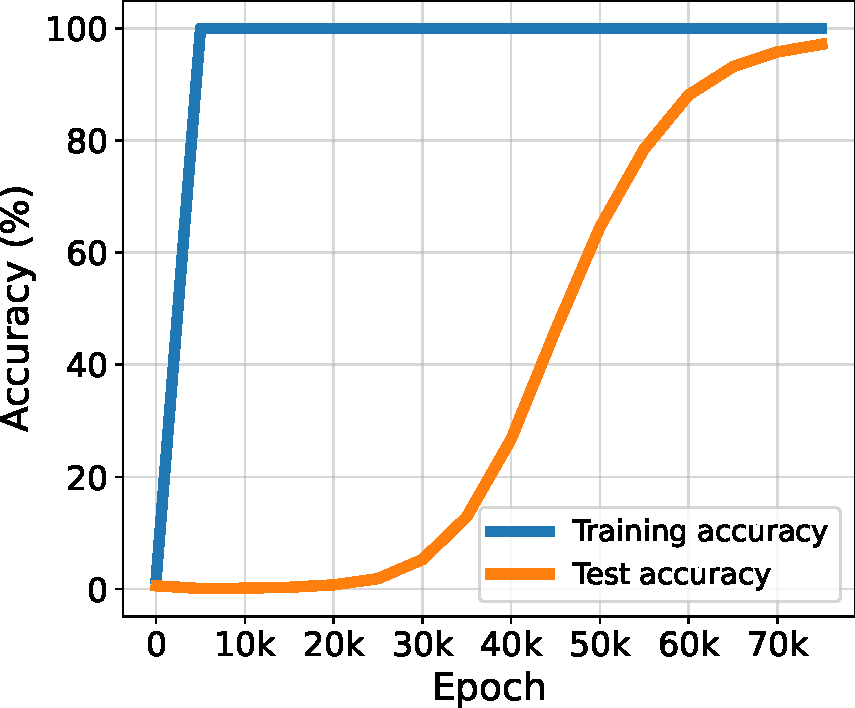
\includegraphics[width=\linewidth]{grokking_iclr/figures/teaser_softermax.pdf}
    \label{fig:input_representations}
    \caption{AdamW + stablemax}
\end{subfigure}%
\hfill
\begin{subfigure}[t]{.32\textwidth}
    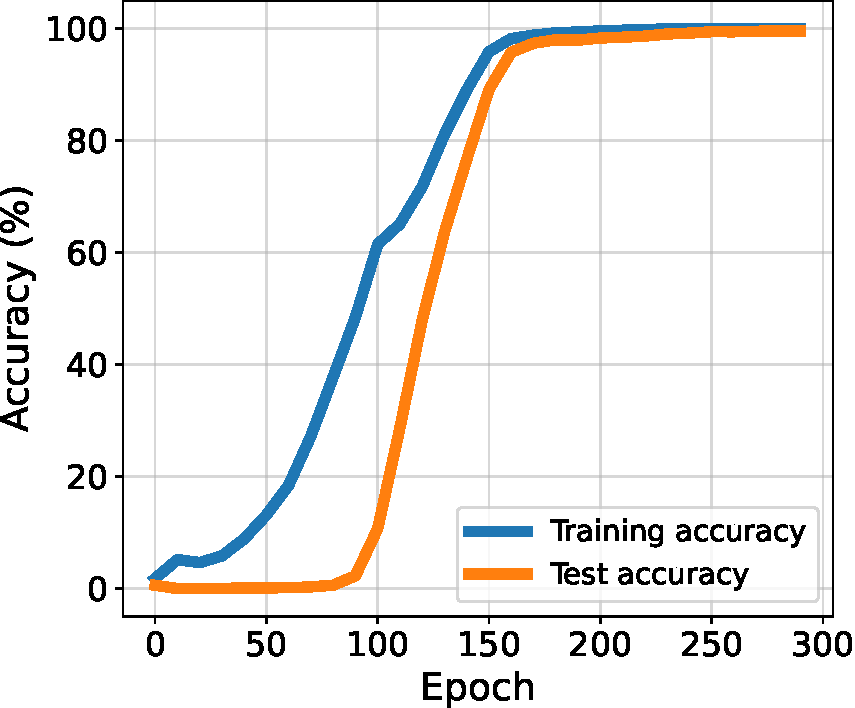
\includegraphics[width=\linewidth]{grokking_iclr/figures/teaser_nlm.pdf}
    \label{fig:gradient_norms}
    \caption{$\perp$AdamW + stablemax}
\end{subfigure}
\caption{\vspace{-5mm}}
\vspace{-5mm}
\end{figure}
\end{comment}
\section{Overview of the approach}
\label{sec:overview}
Fig.~\ref{fig:underlying} describes the underlying process we aim to model:
given a discrete feature map $I[i,j]$, we are interested in constructing \niv{a} CC-layer that operates on $I$ as an input, and produces a next layer $I'[i',j']$, by modeling a learned continuous convolution between the input and output feature-maps.
%$I$ and $I'$. 
Note that the input and output feature-maps  $I$ and $I'$ need \emph{not} be related by an integer  scale factor (or its inverse).
%
Such \niv{an} action can be realized by \niv{the following steps}: 
\vspace*{0.1cm} \\ 
(i)~Use a ''Bed of Nails'' representation of $I$:
$I_{cont}(h,w) = \sum_{i,j}\delta(h-i, w-j)I[i,j]$.
where $i,j$ are discrete `pixel' (feature) locations in $I$, and $h,w$ are continuous coordinates in the continuous feature-map space. 
%For simplicity, we will refer from here on  to all discrete coordinates inside feature maps \niv{(whether input images or the outputs of intermediate network layers)} by the term \textbf{`pixels'}, and their in-between non-integer coordinates as \textbf{sub-`pixel'}. 
For simplicity, {we will refer from here on  to all discrete coordinates inside feature maps by the term \textbf{`pixels'}, and their in-between non-integer coordinates as \textbf{sub-`pixel'} (although we are referring to general network layers; usually not images)}. 
\vspace*{0.1cm} \\
(ii)~Apply a convolution with a \emph{learned} continuous kernel $\mathcal{K}_\theta(h,w)$.
\vspace*{0.1cm} \\
(iii)~Resample the continuous result of the convolution according to the desired shape and scale-factors of $I'$. The resampling grid is purely a function of the shape and scales.
%and the only function of them in the process. 
This means that the same continuous kernel $\mathcal{K}_\theta$ is eligible for producing any desired scale-factor for $I'$.

These phases are indicated in Fig.~\ref{fig:underlying}, and can be mathematically formulated as follows:
\begin{align}
    CC\{I\}[\textbf{n}] = \{I_{cont} * \mathcal{K}_{\theta}\}(\textbf{g}_n)
    &=
   \iint\sum_{\textbf{m}}\delta
   \left(\textbf{g}_n-\mathbf{\tau}-\textbf{m}\right)
    I[\textbf{m}] \mathcal{K}_\theta(\mathbf{\tau})d \mathbf{\tau} \notag\\
    &=
  \sum_{\textbf{m}}I[\textbf{m}]\iint
  \Big(\delta\left(
  \textbf{g}_n-\mathbf{\tau}-\textbf{m}\right)
     \mathcal{K}_\theta(\mathbf{\tau})\Big)d \mathbf{\tau} \notag\\
    % \iintertext{The Dirac Delta function implies that a non-zero contribution only occurs when $\mathbf{\tau}=\textbf{g}_n-\textbf{m}$.} 
   &=\sum_{\textbf{m}}
     I[\textbf{m}]\mathcal{K}_\theta(\textbf{g}_n-\textbf{m})
\label{eq:underlying}
\end{align}



% \niv{alternative for next \underline{two} paragraphs: 
where $\textbf{m}=(i,j),  \textbf{n}=(i',j')$ are discrete `pixel' coordinates in $I$ and $I'$ respectively, and $\textbf{g}_n$ denotes the continuous sampling locations of the grid
in Fig.~\ref{fig:underlying} 
(i.e., the sub-`pixel' position of  each `pixel' in $I'$ when projected onto the coordinates of $I$). 

Eq.~\ref{eq:underlying} shows that for $\mathcal{K}_\theta$ with finite support, the output of the continuous convolution at $I'[\textbf{n}]$ is a weighted sum of the discrete ``Neighbors'' of its projected location  $\textbf{g}_n$ in the input $I$. The weights are a function of the distance between the discrete `pixel' center  $\textbf{m}$  to the continuous sampling location~$\textbf{g}_n$.
%
The desired sampling grid \varbold{$\textbf{g}_n$} is calculated by projecting the output integer `pixel' locations $\textbf{n}=(i',j')$ in $I'$, to sub-`pixel' coordinates in the input $I$. 
We call it the {``Projected Grid''}. 

% Assuming \niv{If?} $\mathcal{K}_\theta$ has finite support, there is a constant number of set of indices $\textbf{m} \in I$ that contribute to $\textbf{n}$ \niv{we've already mentioned it above, though non-rigorously as in here. but better just drop one of them, otherwise it's redundant}. 
% We call these the \textbf{Neighbors} of the projected grid point $\textbf{g}_n$, and denote them by $\varbold{\mathcal{N}\textbf{[n]}}$. Each such set of neighbors has a corresponding 
% set of  learnable \textbf{Weights};
% $\varbold{\mathcal{W}\textbf{}{[n,m]}} = \mathcal{K}_\theta(\textbf{g}_n-\textbf{m})$.
% Once these three tensors are extracted, Eq.~\ref{eq:underlying} can be modeled.


% where $\textbf{n},\textbf{m}$, $\textbf{g}_n$ denote 2D vectors:   $\textbf{m}=(i,j),  \textbf{n}=(i',j')$ are the discrete `pixel'  coordinates in $I$ and $I'$ respectively, and $\textbf{g}_n$ denotes the continuous sampling locations of the grid in Fig.~\ref{fig:underlying} 
%(i.e., the sub-`pixel' position of  each `pixel' $(i',j')\in I'$ \niv{consider removing $(i',j')\\$ as these are coordinates, and also it's enough to just say "in I"} when projected onto the coordinates  of layer $I$).

% Eq.~\ref{eq:underlying} shows that the learned continuous convolution values \niv{maybe "outputs" instead of "values", as it's not clear. readers might confuse values to be either the outputs or the set of weights} are obtained from discrete feature values at `pixel' centers $I[\textbf{m}]$, multiplied by weights which 
% are a function of the distance between the discrete `pixel' center  $\textbf{m}$  to the continuous sampling location $\textbf{g}_n$. 
% In other words, if $\mathcal{K}_\theta$ has a finite support, every output neuron is a weighted sum of the discrete ``neighbors'' of its projected location in the input layer. 


% \section{Method}
\begin{figure}[t]
\vspace*{-1cm}
    \centering
%    \hspace*{-0.5in}
%    \includegraphics[width=1.3\textwidth]{figs/fig_overview.jpg}
    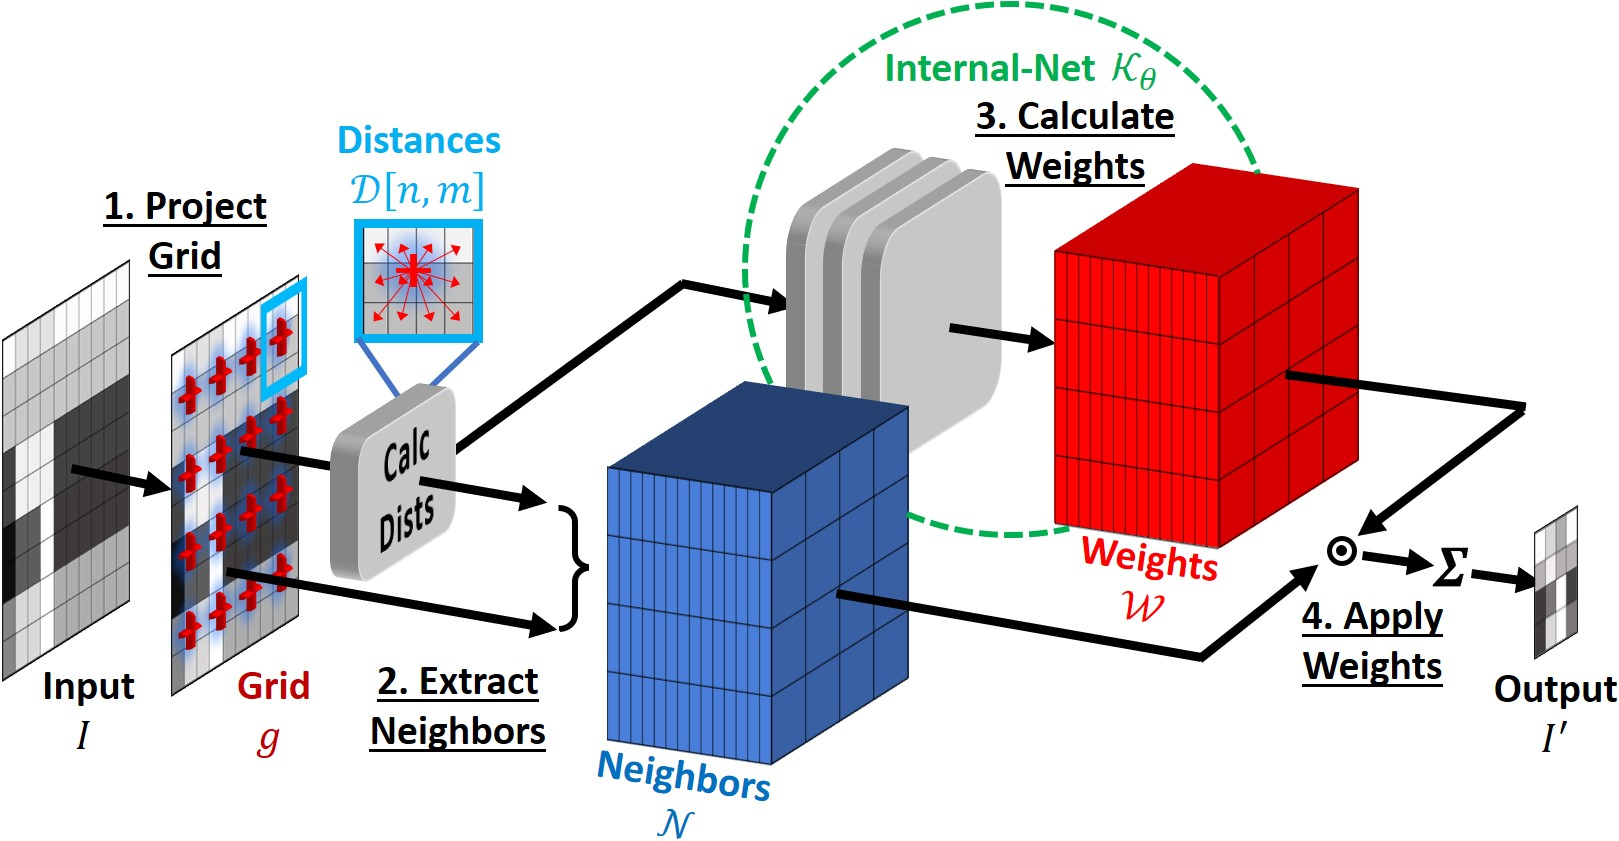
\includegraphics[width=0.9\textwidth]{figs/fig_overview_Ben.jpg}
    \caption{\it Overview of CC-layer. \ (see Sections~\ref{sec:overview} and~\ref{sec:implement} for details)}
    \label{fig:overview}
    \vspace*{-0.3cm}
\end{figure}

%\textbf{CC Overview:} 
% In order to execute our approach we need to overcome an inherent challenge:
% CNNs are built upon regular grids with discrete coordinates. We need to model a continuous process with discrete components. 
%Moreover, the final model needs to be end-to-end trainable by back propagation. \niv{next sentence is redundant} Our proposed construction of the CC-layer extracts all the components of Eq.~\ref{eq:underlying} and executes them.


In order to execute our approach we need to overcome an inherent challenge:
CNNs are built upon regular grids with discrete coordinates. 
We therefore need to model a continuous process with discrete components. 
Fig.~\ref{fig:overview} illustrates our CC-layer construction, which builds upon implementation ideas from standard image resizing techniques~\cite{MATLAB:2010}. 
Our CC-layer consists of 4 principled building blocks. These are marked by numbers in Fig.~\ref{fig:overview}, and are described in detail in Sec.~\ref{sec:implement}: 
\begin{enumerate}[noitemsep,nolistsep,leftmargin=*]
% \item \textbf{Calculate Projected Grid \varbold{$\textbf{g}_n$}:} 
% The desired sampling grid \varbold{$\textbf{g}_n$} is calculated by projecting the output integer `pixel' locations $\textbf{n}=(i',j')$ in $I'$, to sub-`pixel' coordinates in the input $I$. 
%We call it the \textbf{Projected Grid}. 
\item \textbf{Calculate Projected Grid \varbold{$\textbf{g}_n$}} 
from the desired scale-factors and  output-shape. 
% This is done both at train and at test time.
\item \textbf{Extract Neighbors \varbold{${\mathcal{N}}$}:} Map each sampling point $\textbf{g}_n$ to its discrete neighbors \varbold{${\mathcal{N}}[\textbf{n}]$} within the continuous kernel support. 
% This is done both at train and at test time.
\item \textbf{Calculate Weights} \varbold{$\mathcal{W}$} by applying \textbf{$\mathcal{K}_\theta$} to distances between sampling points to their neighbors:
$\varbold{\mathcal{W}\textbf{}{[n,m]}} = \mathcal{K}_\theta(\textbf{g}_n-\textbf{m})$.
%This is the only learnable part (learned at train-time). 
This ``Internal-Net''  \textbf{$\mathcal{K}_\theta$} is the only trainable part in the CC-layer.
%also the only part of the CC-layer that is kept in memory during train and test time. 
%\textbf{\textcolor{red}{Please circle Internal-Net in Fig2 by a green dashed line and add in green: \textcolor{cyan}{Internal-Net  \textbf{$\mathcal{K}_\theta$}}}}
\item \textbf{Apply Weights:}  Multiply \varbold{$\mathcal{N} \odot \mathcal{W}$} and sum over all neighbors and input channels, to obtain the output \ben{feature map} $I'$, with any desired scale or shape (which can be determined at test time).
\end{enumerate}

% Sec.~\ref{sec:implement}  describes in detail each of these four CC blocks, and explains how to train the dynamic CC-layer to allow for dynamic scale-generalization at test time. Sec.~\ref{sec:features} reviews the properties and benefits of the CC-layer, and presents new approaches for \emph{dynamic architectural design}, which become possible with the new CC-layer.  In Sec.~\ref{sec:efficiency} we specify ways to efficiently train CC. Finally, Sec.~\ref{sec:applications}  showcases a few possible ways to exploit CC-layers in various Computer Vision tasks. 
% \assaf{I would drop this paragraph}
% \michal{I agree}
%---------------------------------
\vspace{-0.6em}
\section{Method}
\label{sec:method}
%---------------------------------

We propose a method to equip pre-trained Text-to-Video (T2V) models with a style adapter, allowing for the generation of stylized videos based on both a text prompt and a style reference image. The overview is illustrated in Figure~\ref{fig:overview}. In this framework, the textual description dictates the video content, while the style image governs the visual style, ensuring a disentangled control over the video generation process.
Given the limited availability of stylized videos, we employ a two-stage training strategy. Initially, we utilize an image dataset abundant in artistic styles to learn reference-based style modulation. Subsequently, adaptation finetuning on a mixed dataset of style images and realistic videos is conducted to improve the temporal quality of the generated videos.


%
\begin{figure}[t]
    \centering
    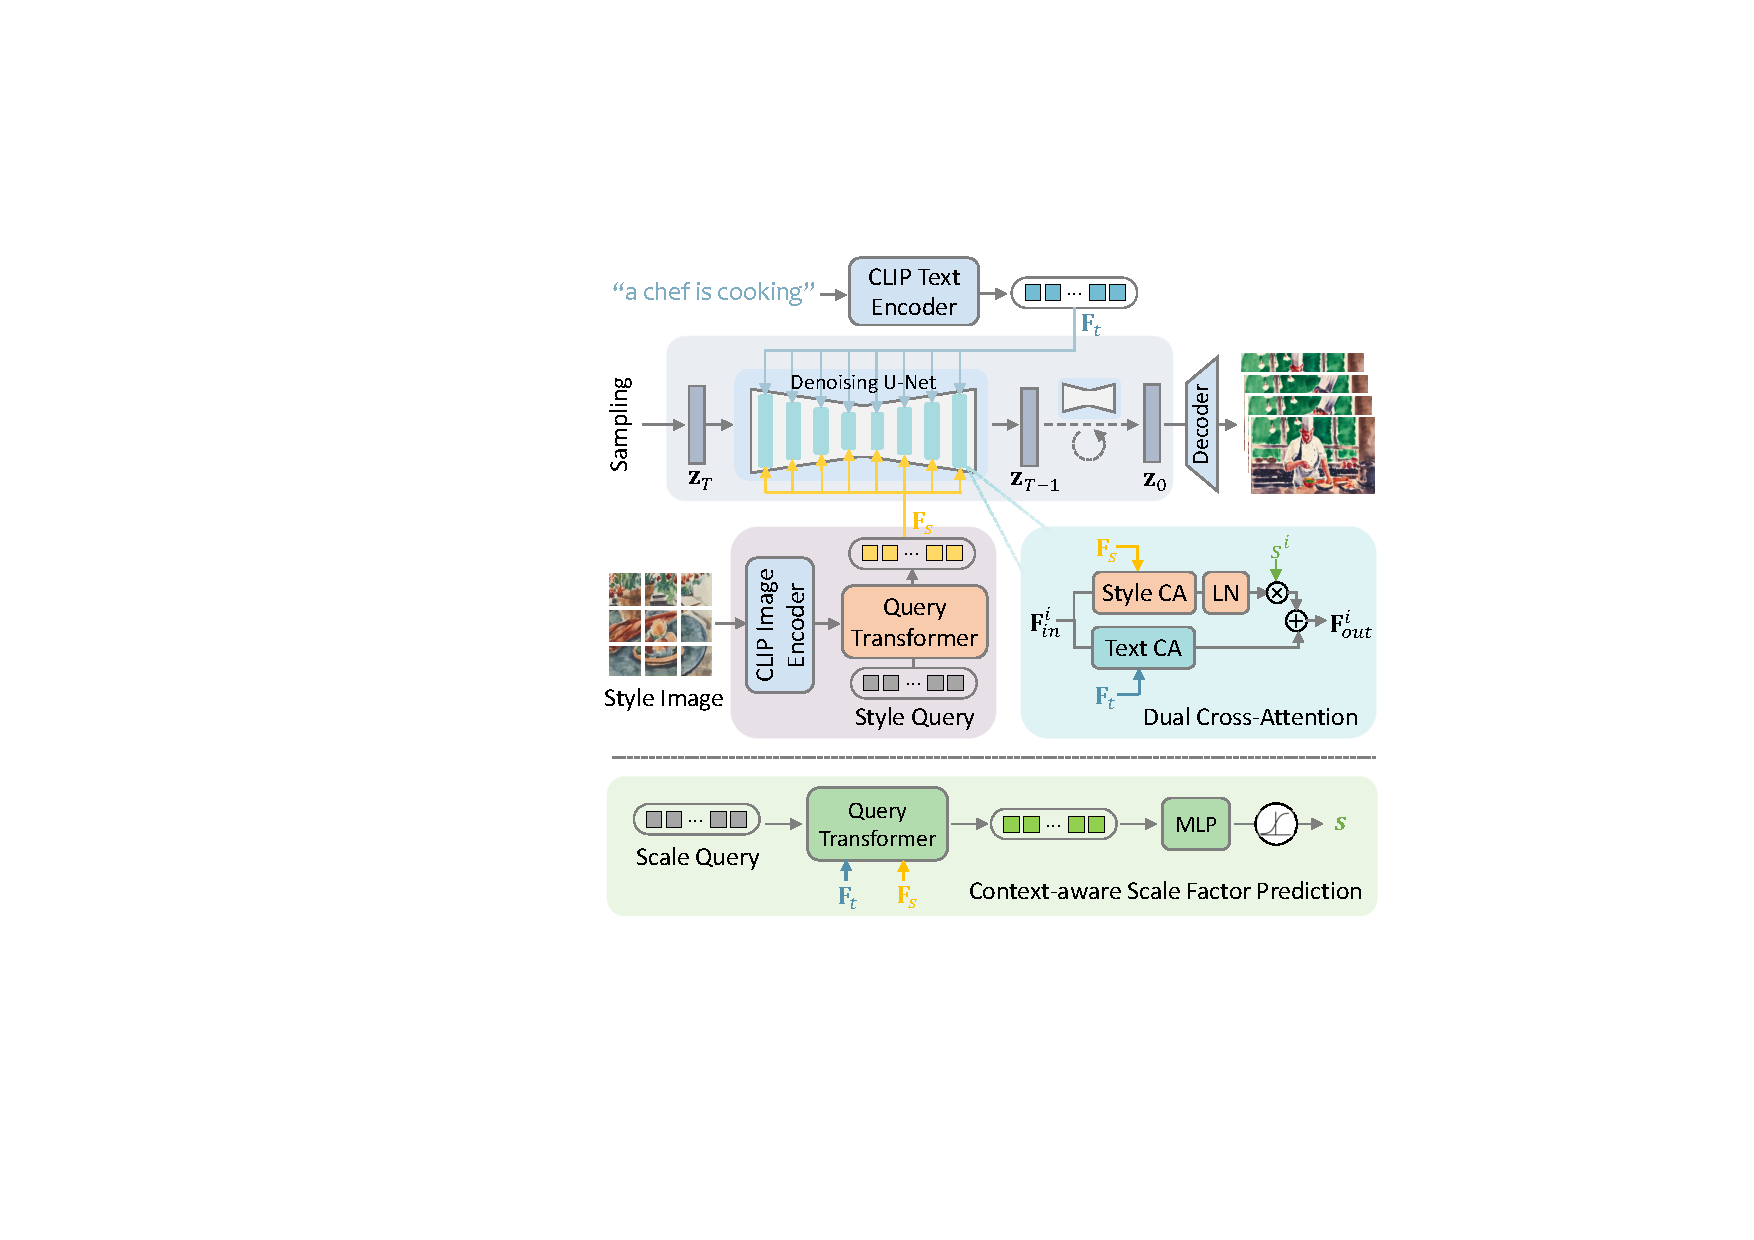
\includegraphics[width=0.95\linewidth]{figures/overview2.pdf}
    \vspace{-0.35cm}
    \caption{Overview of our proposed style adapter. It consists of three components, i.e. style feature extractor, dual cross-attention module, and context-aware scale factor predictor.}
    \label{fig:overview}
    \vspace{-1.4em}
\end{figure}


%---------------------------------
\vspace{-0.6em}
\subsection{Reference-Based Style Modulation}
\label{subsec:style_modulation}
%---------------------------------

Our style adapter serves to extract style features from the input reference image and infuse them into the backbone features of the denoising U-Net. As mainstream T2V models~\cite{chen2023videocrafter, chen2024videocrafter2, wang2023modelscope, wang2023lavie} are generally initialized from open-source T2I Models and trained with image and video datasets in a joint strategy, they support not only text-to-video generation but also retain the capacity for text-to-image generation. To overcome the scarcity of stylized videos, we propose to train the style adapter based on a pre-trained T2V model (i.e. VideoCrafter~\cite{chen2023videocrafter}) for stylized image generation under the supervision of stylistic images.

\vspace{-0.3em}
\paragraph{Content-Style Decoupled Data Augmentation.}
\label{sec:data_aug}
We use the stylistic images from two publicly available datasets, i.e. WikiArt~\cite{phillips2011wiki} and a subset of Laion-Aesthetics~\cite{schuhmann2022laion} (aesthetics score above 6.5). In the original image-caption pairs, we observe that the captions generally contain both content and style descriptions, and some of them do not match the image content well. To promote the content-style decoupling, we use BLIP\nobreakdash-2~\cite{li2023blip2} to regenerate captions for the images and remove certain forms of style description (e.g., \textit{a painting of}) with regular expressions.
In addition, as an image contains both style and content information, it is necessary to construct a decoupling supervision strategy to guarantee the extracted style feature free of content features. Although a stylistic image may contain different local style patterns~\cite{park2019arbitrary, huo2021manifold, chen2023tssat}, we regard that a large crop of an image(e.g. 50\% of the image) still preserves a similar style representation with the full image.
% We regard that every local regions of a stylistic image share the same style representation, which not only reflects on texture and color theme but also on the structure and perceptual semantics. 
Based on this insight, we process each stylistic image to obtain the target image and style image through different strategies: for target image, we scale the shorter side of the image to 512 and then crop the target content from the central area; for style image, we scale the shorter side of the image to 800 and randomly crop a local patch with $512 \times 512$. This approach reduces the overlap between the style reference and generation target, while still preserving the global style semantics complete and consistent.

\vspace{-0.3em}
\paragraph{Style Embedding Extraction.}
CLIP~\cite{radford2021learning} has demonstrated remarkable capability in extracting visual features from open-domain images. To capitalize on this advantage, we employ a pre-trained CLIP image encoder as a feature extractor. Specifically, we utilize both the global semantic token and the full $256$ local tokens (i.e., from the final layer of the Transformer) since our desired style embedding should not only serve as an accurate style trigger for the T2V model, but also provide auxiliary feature references.
As image tokens encompass both style and content information, we further employ a trainable Query Transformer (Q-Former)~\cite{li2023blip2} to extract style embedding $\mathbf{F}_s$. We create $N$ learnable style query embeddings as input for the Q-Former, which interact with image features through self-attention layers.
%We define style as the synthesized information present in an image that characterizes its overall aesthetic, independent of content. It encompasses both high-level aesthetic semantic information, such as composition, artistic conception, and color scheme, as well as low-level texture information, including specific brush stokes, lines, and surface details.
Note that this is a commonly adopted architecture for visual condition extraction~\cite{li2023blip2, shi2023instancebooth,ye2023ipadapter, xing2023dynamicrafter}. But it is the style-content fusion mechanism that makes our proposed design novel and insightful for style modulation, as detailed below.

\begin{figure}[t]
    \centering
    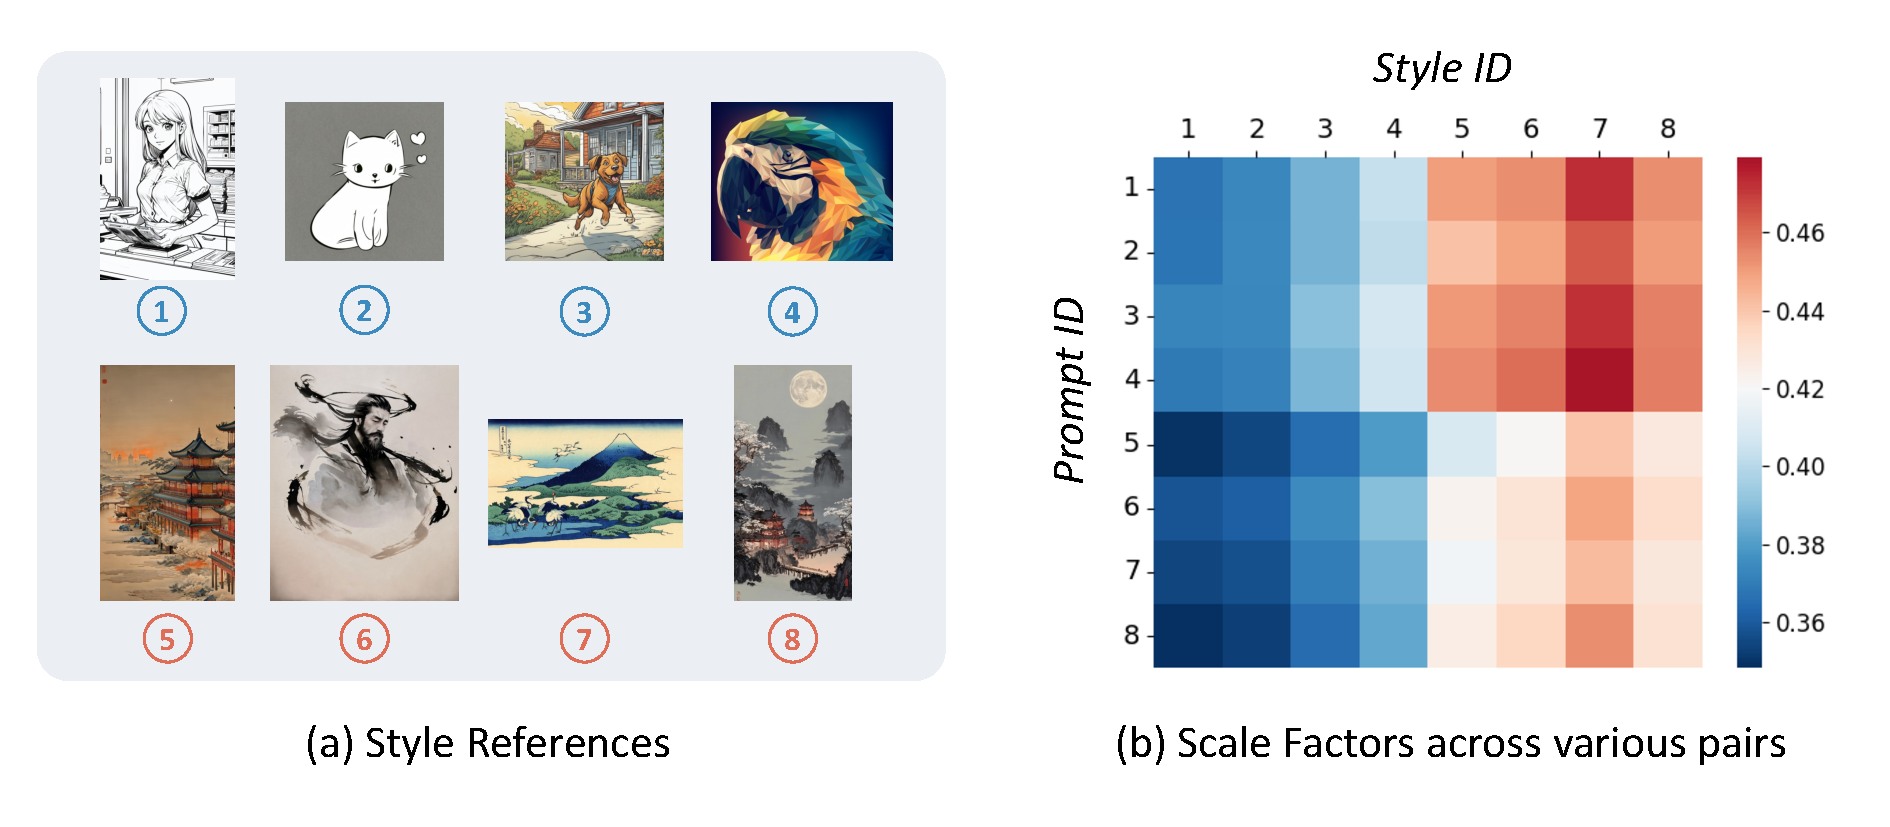
\includegraphics[width=\linewidth]{figures/scale_factor_viz.pdf}
    \vspace{-1.0cm}
    \caption{Illustration of content-style fusion scale factors across multiple input pairs. Four short prompts(less than 5 words) with prompt id $\in [1, 4]$ and four long prompts(more than 8 words) with prompt id $\in [5, 8]$ are randomly selected. Results indicate that shorter prompts and images with richer style-semantics tend to have relatively higher scale factors.} 
    \label{fig:scale_factor_viz}
    \vspace{-0.35cm}
\end{figure}

\paragraph{Adaptive Style-Content Fusion.}
\label{sec:fusion}
With the extracted style embedding, there are two ways to combine the style and text conditions, including (i) \textit{attach-to-text}~\cite{composer,gligen,ramesh2022hierarchical}: attach the style embedding to the text embedding and then interact with the backbone feature via the originally text-based cross-attention as a whole; (ii) \textit{dual cross-attention}~\cite{wei2023elite,ye2023ipadapter}: adding a new cross-attention module for the style embedding and then fuse the text-conditioned feature and style-conditioned feature.
According to our experiment (see Sec.~\ref{subsec:ablation}), solution (ii) surpasses solution (i) in disentangling the roles of text and style conditions, therefore we have adopted it as our final solution. The formula can be written as:
\vspace{-0.3em}
\begin{equation}
    \mathbf{F}_{out}^{i} = \text{TCA}(\mathbf{F}_{in}^i, \mathbf{F}_t) + s^i * \text{LN}(\text{SCA}(\mathbf{F}_{in}^i, \mathbf{F}_s)),
\end{equation}
where $\mathbf{F}_{in}^i$ denotes the backbone feature of layer $i$, LN denotes layer normalization, and TCA and SCA denote text-based cross attention and style-based cross attention respectively. $s^i$ is a scale factor learned by a context-aware scale factor prediction network, to balance the magnitudes of text-based feature and style-based feature.
The motivation is that different stylistic genres may have different emphasis on content expression. For example, the abstract styles tend to diminish the concreteness of the content, while realism styles tend to highlight the accuracy and specificity of the content. So, we propose a context-aware scale factor prediction network to predict fusion scale factors according to the input contexts.
Specifically, we create a learnable factor query, it interacts with textual features $\mathbf{F}_t$ and style features $\mathbf{F}_s$ to generate scale features via a Q-Former and then project it into layer-wise scale factors $\mathbf{s} \in \mathbb{R}^{16}$.
Figure~\ref{fig:scale_factor_viz} illustrates the learned scale factors across multiple contexts. It shows that the adaptive scale factors have a strong correlation with style genres while also depending on the text prompts. Style references with rich style-semantics(i.e., ukiyo-e style) typically yield higher scale factors to emphasize style; while complex prompts tend to produce lower scale factors to enhance content control.  This is consistent with our hypothesis to motivate our design.


%---------------------------------
\vspace{-0.5em}
\subsection{Temporal Adaptation to Stylized Features}
\label{subsec:temp_adaptation}
%---------------------------------

Given a pre-trained T2V model, the style adapter trained on image dataset works well for stylized image generation. However, it still struggles to generate satisfactory stylized videos, which is vulnerable to temporal jittering and visual artifacts.
The possible causes are that the cross-frame operations, i.e. temporal self-attention, do not involve in the process of stylized image generation, and thus induce incompatible issues. So, it is necessary to finetune the temporal self-attention with the style adapter incorporated.
Following the practice of T2V image and video joint training, the finetuning is performed on the mixed datasets of stylistic images and photorealistic videos. This is an adaptation training of temporal blocks while the other modules remain frozen, and the model converges efficiently.

\vspace{-0.5em}
\paragraph{Classifier-Free Guidance for Multiple Conditions.}
Unlike T2I models, video models exhibit a higher sensitivity to style guidance due to their limited stylized generation capabilities. Using a unified $\lambda$ for both style and context guidance may lead to undesirable generation results. Regarding this, we adopt a more flexible mechanism for multiple conditions classifier-free guidance. Building upon the vanilla text-guided classifier-free guidance, which controls context alignment by contrasting textual-conditioned distribution $\epsilon(z_t, c_t)$ with unconditional distribution $\epsilon(z_t, \varnothing)$, we introduce the style guidance with $\lambda_s$ by emphasizing the difference between the text-style-guided distribution $\epsilon(z_t, c_t, c_s)$ and the text-guided distribution $\epsilon(z_t, c_t)$. The complete formulation is as below:
\begin{equation}
    \begin{aligned}
        \hat{\epsilon}(z_t, c_t, c_s) = \epsilon(z_t, \varnothing) &+ \lambda_s(\epsilon(z_t, c_t, c_s) - \epsilon(z_t, c_t)) \\
        &+ \lambda_t(\epsilon(z_t, c_t) - \epsilon(z_t, \varnothing)),
    \end{aligned}
\end{equation}
where $c_t$ and $c_s$ denote textual and style condition respectively. $\varnothing$ denotes using no text or style conditions.
In our experiment, we follow the recommended configuration of text guidance in VideoCrafter~\cite{chen2023videocrafter}, setting $\lambda_t = 15.0$, while the style guidance is configured with $\lambda_s = 7.5$ empirically. Similarly, we set $\lambda_t = 7.5$ and $\lambda_s = 5.0$ for style-guided image generation.






\section{Features \& Properties}
\label{sec:features}
This section reviews several important and useful properties of CC.
%and mostly new possibilities to CNN architecture design introduced by CC.
We show that introducing CC-layers gives rise to new CNN capabilities, and furthermore -- allows for \emph{new dynamic architectural designs determined at inference time}.

\textbf{A standard Conv-layer is a special case of the CC-Layer:}
Note that when the scale-factor $s=\nicefrac{1}{k}$, $k \in \mathbb{N}$, and $k$ has the same parity as the kernel support size in both dimensions, $g_n$ in Eq.~\ref{eq:grid} reduces to simple grid locations with integer pixel spacing between them. Thus, all output grid points share the same set of local distances to their discrete input ``Neighbors''. Hence, the set of weights are shared by all output `pixels', which is the case in standard convolution. This implies that  for integer scale ratios CC reduces to standard convolution, i.e.,  CC is a \emph{generalization} of the standard Conv-layer.

% \textbf{Collapsing back to standard convolution:} First we note that the distance of a grid point to the closest pixel center in the input determines the distances to all neighbors. This means that grid locations with same distance to closest `pixel' center share the same distances to neighbors and consequently will be mapped to the same set of weights. Considering this, we note that eq.~\ref{eq:grid} suggests that there are special cases. A scale-factor that is inverse of integer in both dimensions, produces grid locations with full `pixels' spacing between them, thus they all share the same distance to closest `pixel' center. As explained, the set of weights for each output `pixel' in such situations is identical. This implies that CC for such scale is actually a standard convolution, and shows that CC is a generalization of standard conv-layer.

\textbf{Dynamic scale-factor at inference:} As mentioned, the projected-grid is purely a function of the scale-factors and output shape. It is also important to note that in case of training the CC-layer with a \emph{random float scale factor}, we obtain a huge diversity of distances in $\varbold{\mathcal{D}}$ (see more details in Sec.~\ref{sec:train}). Hence the ``Internal-Net'' $\varbold{\mathcal{K}_\theta}$ which gets all the sub-`pixel' distances $\varbold{\mathcal{D}}$ as an input, and outputs a single kernel  consistent with them all,  must learn a  \emph{true continuous} weight function (the continuous kernel), independently of the scale factor or shape of the \ben{output}. Once it has recovered the continuous kernel (continuous weights),  CC can be applied at inference time to output any dynamically chosen scale or shape, simply by changing the sampling grid.

% \textbf{Cross-scale generalization:} Since the learning model $\mathcal{K}_\theta$ is unaware of the scale, it can be trained to one scale and generalize to another, under reasonable conditions. the scale trained on, cannot be a special case that collapses back to convolution, or a rational number with a denominator that is too small. In other words, generalization occurs over the distribution of distances between the grid and `pixel' centers. If this distribution collapses to a small set of possibilities then such generalization is damaged. A randomly selected float scale-factor will be able to generalize with probability ~1. 

\textbf{True Shift-Invariance/equivariance:} It was shown~\cite{zhang2019shiftinvar, azulay2018deep} that strided conv-layers \niv{lack}
% have damaged 
equivariance to shifts of the \ben{input}. This mostly happens due to aliasing. The common filter size tends to be smaller than the low-pass filter size required to remove high-frequencies when downscaling by a factor of 2. CC allows more gradual downscaling, so that (with the same kernel support) the sampling frequency is higher and less aliasing occurs. For example, one can replace a single strided convolution layer with downscaling-factor $s=1/2$, with a few (2-3) CC-layers, each with scale $1/2 < s < 1$ (e.g., 2 CC-layers with $s=1/\sqrt{{2}}$, or 3 CC-layers with $s=1/\sqrt[3]{{2}}$).

\textbf{Standard conv-layers often suffer from inherent misalignments, which are ameliorated by CC-layers:} Examining the accurate grid mapping in Eq.~\ref{eq:grid}, one can see that there are cases in standard discrete convolutions which fail to satisfy it. Such cases occur when the size of the filter and the stride have different parities, in some dimension. The intuitive reason is that the filter \emph{center} is defined by its parity: In odd-sized filters, the center of the output `pixel' falls on an input `pixel'-center, whereas in even-sized filter, it falls on the boundary between two input `pixels'. As mentioned, for a scale factor $1/int$, the set of weights is identical for any output position. Eq.~\ref{eq:grid} suggests that in such cases the grid locations are either all exactly on input `pixel' centers, or all on the boundary between input `pixels' (e.g., scale-factor of $\frac{1}{2}$ produces locations 0.5, 2.5, 4.5 etc., whereas scale factor of $\frac{1}{3}$ produces locations 1,4,7 etc.) This means that in case of an even scale with odd-sized filter, standard conv-layers introduce small misalignments between the input and output ($I$,$I'$). These small \benc{del: layer-to-layer} misalignments can accumulate to large misalignments over many layers. 

Such an example is shown in Fig.~\ref{fig:fig_missalign}. 
% Applying a fixed kernel for which the center of mass is the filter center, with a parity different than the scale will shift the result by half a `pixel'. Fig.~\ref{fig:fig_missalign} shows a simple experiment. 
We used a simple gaussian kernel,  and applied it repeatedly to an input image (white cross), using either a sequence of standard conv-layers or a sequence of CC-layers, all with stride=1 or scale=1, respectively. We chose an even-sized 4$\times$4 kernel. It can be seen that standard conv-layer shifts the result by half a pixel per iteration, resulting in a large shift after many iterations. In contrast, CC-based convolutions remain centered, due to the accurate sub-pixel grid mapping of Eq.~\ref{eq:grid}. Choosing a different padding method for the standard conv would only result in shifts to other directions; there is no way to apply a 4$\times$4 discrete convolution that keeps the same input size and does not induce misalignments. The reason neural networks still get good results is simple: they learn a variety of shifted kernels. This misalignment phenomenon has been observed in super-resolution works~\cite{zhang2020deep, ZSSR}. Still, the way  misalignments are currently addressed is non-ideal and unprincipled, as some portion of the filter size is not used and may create artifacts.

\textbf{Scale Ensembles:} Here we present \niv{an entirely}
% a totally 
new capability in Deep-Learning -- Dynamic Architectural Design of CNNs, at inference time, which is made possible by introducing multiple CC-layers into CNNs.  As mentioned before, a trained CC-layer can generate any output scale-factor chosen at inference time. Therefore, a single trained CNN which consists of multiple CC-layers, can be applied many times at inference, each time with \emph{a different sequence of scales}, as long as the final output scale \& shape of the entire network remain fixed. This means that there are infinitely many ways to apply such a trained network, and still get the same final output size/scale.  Moreover, each dimension (vertical or horizontal) can be scaled differently at intermediate CC-layers. This gives rise to a new type of ``self-ensembles'' of CNNs. We call it ``Scale Ensembles''.  Fig.~\ref{fig:scale_ensemble} schematically illustrates a few different scales-sequences for 3 consecutive CC-layers in the same pre-trained CNN. For example, the Green sequence applies 3 consecutive uniform scaling in both dimensions, same scaling each time; 
%, and uses a larger scale as the last one. 
the Blue sequence scales  the horizontal and vertical dimensions alternatingly; whereas the Red sequence offers yet another non-uniform sequence of scaling. At inference time we can apply the same pre-trained network several times, each with a different sequence of scales. We can then aggregate all the results of this ensemble,  to get an improved result  which is consistent with the entire ensemble. Aggregation can be achieved, e.g., by  averaging the class \niv{logits}
% probabilities 
in a classification task,  or by computing the median image of the ensemble in an image-processing task.

\begin{figure}
%\vspace*{-0.5cm}
\hspace{-0cm}
\centering
\begin{minipage}{.45\textwidth}
    \hspace{-1cm}
    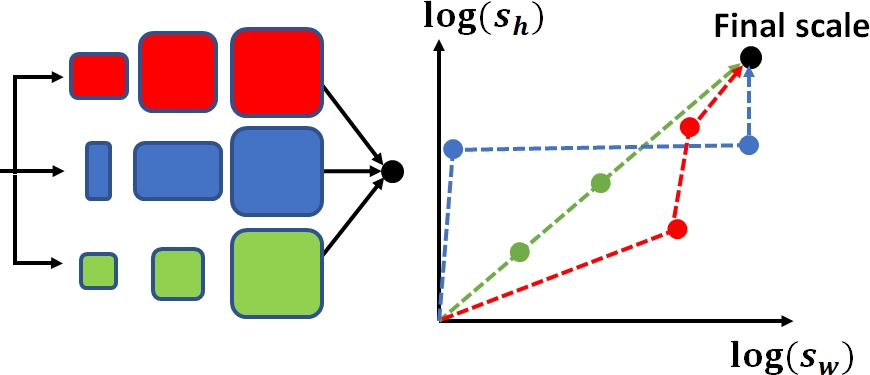
\includegraphics[width=1\textwidth]{figs/fig_scale_ensemble_Michal.jpg}
    \captionsetup{oneside, margin={-2cm,0cm}}
     \caption{\it ``Scale-Ensemble'' (see Sec.~\ref{sec:features}  for details).}
    \label{fig:scale_ensemble}
\end{minipage}%
  \hspace{0.3cm}
  \begin{minipage}{.3\textwidth}
  \centering
  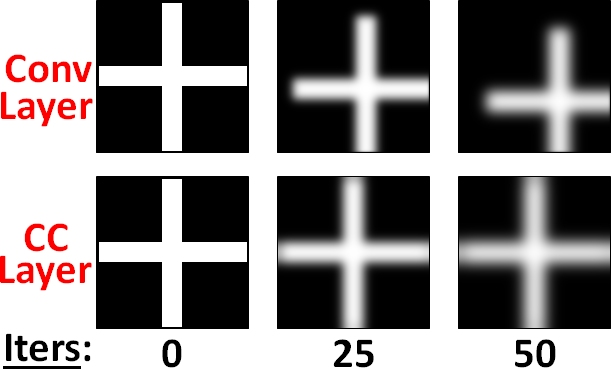
\includegraphics[width=1\textwidth]{figs/fig_misalign_Michal.jpg}
   \captionsetup{oneside, margin={-0.5cm,-1cm}}
  \caption{\it Standard conv-layers induce misalignments.  CC-layers do not.}
  \label{fig:fig_missalign}
    \end{minipage}
   \vspace*{-0.5cm}
\end{figure}
\section{Efficient Implementation}
\vspace{-0.3cm}
\label{sec:efficiency}
This section provides major implementation details which give rise to efficient implementation of the CC-layer. Code will be made available.
% Other details and performance analysis can be found in the supplementary material. \michal{Will we have SuppMaterial?}
%We may need to, given that we already have an excess of 1 page (and the experiments section is not fully written yet...)  But if not, we should make sure to remove this sentence.}

\textbf{No need to keep the Neighbors distances:} The distances $\varbold{\mathcal{D}}$  of a grid point  \varbold{$\textbf{g}_n$}  to all its discrete input Neighbors can actually be predicted by keeping only one Neighbor. The reason is simple: all neighbors are at a sequence of positions 1 `pixel' apart from each other. 
It suffices to keep only the distance of a grid point to its \emph{closest} `pixel' center in order to predict all other distances. Moreover, the distance to each Neighbor is already implied by the sub-`pixel' grid coordinates. Hence, we can train the Internal-Net
$\varbold{\mathcal{K}_\theta}$  to predict the weights \emph{directly from the grid} \varbold{$\textbf{g}$}, thus saving on memory. 

% \textbf{Efficient implementation using discrete convolutions:} Eq.~\ref{eq:grid} 
% suggests that special types of grids exist. We have already noted that for $1/int$ scales, CC collapses to a standard convolution. However, the equation further suggests that for any  scale-factor which is a \emph{rational-number} ($s=k/l$) the grid is periodic, where the period is the numerator $k$. This is a generalization of previous observations made by~\cite{romano2016raisr} and~\cite{freedman2011image}. We take advantage of this property: When the scale-factor is a rational number, with a numerator not too small (to allow for scale generalization), but not too large (to allow for efficient convolutions), we can calculate the sets of weights for one period only. We do not need to explicitly extract neighbors. Instead we use a set of standard discrete convolution filters, each with a different starting shift matching a different grid position within one period. We apply them to the input image and interleave their results. This allows us to use the existing, highly optimized, implementation of conv operation, and also avoid calculation of a huge weights tensor $\mathcal{W}$.

\textbf{Efficient implementation using discrete convolutions:} Eq.~\ref{eq:grid} 
suggests that special types of grids exist. We already noted that for $1/int$ scales, CC collapses to a standard convolution. However, Eq.~\ref{eq:grid}  further suggests that for \emph{rational-numbers}  scale-factors ($s=\nicefrac{k}{\ell}$) the grid is periodic, with a period equals the numerator $k$. This generalizes observations made by~\cite{romano2016raisr,freedman2011image}. We take advantage of this property by calculating the sets of weights for one period only, to avoid calculation of a huge weights tensor $\mathcal{W}$. We do not need to explicitly extract neighbors and multiply them with the weights. Instead, we use a set of standard discrete convolution filters, each with a different starting shift matching a different grid position within one period. We apply them to the input feature-map and interleave their results. This allows us to use the existing, highly optimized, implementation of conv operation. This approach offers a trade-off between speed (small $k$) and better generalization (large $k$). \nivc{the unattentive reviewer might understand from this section that all we do is use a grid of convs instead of one conv. we need to somehow emphasize that this grid can principally change at each iteration, unlike ordinary conv-grids}

% To account for the tradeoff between scale-generalization and efficient convolutions, we take the following 2 precautions: (i)~we choose our scale-factors to be rational numbers with a numerator $\approx 19$ (an irreducible fraction, e.g., 19/27, 19/100, 19/10), thus guaranteeing enough sub-`pixel' distance diversity in the grid, and (ii)~we train the CC-layer with a variety of rational numbers, to further guarantee this diversity.
% To account for the tradeoff between scale-generalization and efficient convolutions, we choose our scale-factors to be rational numbers with a numerator $\approx 19$ (an irreducible fraction, e.g., 19/27, 19/100, 19/10), thus guaranteeing enough diversity of sub-`pixel' distances  in the grid. \ben{I think it should be denominator, not numerator}


\textbf{Saving memory by keeping only $\mathcal{K}_\theta$:} The most memory consuming tensor in CC is the weights tensor $\mathcal{W}$. The second one is the Neighbors tensor $\mathcal{N}$. We can save almost all the memory used by a CC-layer by simply removing these tensors at each iteration after the output is calculated. In the back-propagation step we simply recalculate them, \ben{at some extra cost of time. The memory footprint can be further reduced by chunking the input and computing the per-chunk results sequentially}.
% at a minor extra cost of time (less than 10\%). 
%\ben{this trick can be used in other scenarios} 
%We also conceptually find this as the right way to save the CC layer down the stream; a layer is distinguished by its continuous kernel model  (Internal-Net) $\mathcal{K}_\theta$, 
%and not by the final weights calculated. 
\section{Experiments}
\vspace{-0.3cm}
\label{sec:applications}
% This section presents experiments which exemplify the CC properties discussed  in Sec.~\ref{sec:features}. It further proposes potential use-cases of CC in various Computer Vision applications.

\textbf{Visualizing the continuous learned kernels $K_\theta$:} Filters of discrete conv-layers can be easily visualized. They are sets of discrete numbers on a regular grid, which can just be printed out or viewed as images. Filters of CC-layers, on the other hand, assign a unique set of numbers to any sub-`pixel' grid location. But once trained,
%the Internal-Net $K_\theta$ is trained, 
we can easily sample $K_\theta$ on a regular grid at any desired resolution for the purpose of visualization. Fig.~\ref{fig:visualize} shows 2 such examples of CC kernel visualization. In both examples we trained a single CC-layer to \emph{imitate} an image-resizing method (for which we know the ground-truth kernels): (i) Imitate bicubic resizing, and (ii) imitate resizing by a Gaussian kernel with different $\sigma$ for each axis, rotated by~\ang{45}.  The CC-training was performed  on a single image with a single random sampled scale $s$$\in$$[0.3$$,..,$$1.3]$ in each dimension. The input to the CC-layer was the single image, and the ``output label'' was the resized image  (generated by the external image-resizing method for that $s$).  
%We tested it for: (i)~the well known bicubic resizing; and (ii) a non-isotropic interpolation method -- a Gaussian with different $\sigma$ for each axis, rotated by~\ang{45}. 
Once trained, we sampled $K_\theta$ at dense 200$\times$200 coordinate-pairs.  Fig.~\ref{fig:visualize} shows such visualizations of the  continuous recovered kernel $K_\theta$,  as a function of the training iteration.
%, showing good convergence to the correct ground-truth continuous kernel.

\textbf{Verifying  scale generalization:} To test generalization across scales, we sampled a \emph{single}  pair of random scale-factors $s_x$,$s_y$$\in$$[0.3$$,..,$$1.3]$, and applied an independent bicubic resizing to a single image for this scale. As before, we trained a CC-layer with the original image as  the input, and the resized image as the ``output label''. To test generalization, we applied our CC-layer  (which was {trained} for one scale), on 100 \emph{new random scales}. We compared the resulting 100 output images to ground-truth bicubic resizing by those 100 scales. The left side of Fig.~\ref{fig:generalize} shows  MSE of the train-error and the generalization (test) error. The test-error for scales CC never trained for, is very close to the train-error for the single scale it trained on. This is due to the fact that CC generalizes well to other scales, as long as the training scale generates sufficient diversity in sub-`pixel' grid shifts. To further confirm this, we repeated the experiment, only this time we chose the training scale to be $1/int$ (1/2). Eq.~\ref{eq:grid} shows that in such case all grid locations have the same shift from `pixel' centers (0.5). The right side of Fig.~\ref{fig:generalize} shows that generalization was severely damaged; test-error for 100 other scales was 2-orders-of-magnitude higher. Fig.~\ref{fig:generalize} further shows visualization of $\mathcal{K}_\theta$ for these 2 experiments (ground-truth can be found in Fig.~\ref{fig:visualize}). In the first experiment the learned kernel is similar to the ground-truth, whereas in the second experiment it
is not (since it was only required to produce correct results for a very small subset of coordinate pairs).



% \textbf{Exploiting CC for image classification -- the power of dynamic Scale-Ensembles at inference time:}
% To demonstrate the potential use of CC-layers in
% %that replacing standard conv-layers by CC-layers may improve 
% image classification tasks, we did the following simple experiment:
% We used a variant of a very simple CNN-based classification net for CIFAR-10~\cite{CIFAR10} (similar to the net used in~\cite{wong2018scaling, atzmon2019controlling}). The network consisted of several conv-layers of strides 1,2,1,1,1,2, followed by 3 fully-connected layers, all with ReLU activations. We call this the ``Baseline Net''.

% We construct a ``CC-Classifier'' 
% with the same number of layers, but with CC-layers of \emph{gradually} changing scale factors (starting from the second layer), so that the overall scale factor from the net's input to the last conv-layer's output remains the same (1:4).  
% %At each training iteration a sequence of scale-factors whose \emph{product} yields the global scale factor $\nicefrac{1}{4}$ is randomly sampled  (as in Fig.~\ref{fig:scale_ensemble}). 
% A sequence of scale-factors whose \emph{product} yields the global scale factor $\nicefrac{1}{4}$ is randomly sampled for training the network. 
% %
% %The resulting network gave a pronounced improvement in classification accuracy (+1.4\%).
% %To isolate the impact of the higher number of params in our CC-layers, we further tested a ``CC-baseline'' classifier, which has the same integer scales and strides as in the regular Baseline-Net.
% %All 3 networks were trained in parallel, on same batches with same conditions.
% Both  networks were trained in parallel, on same batches with same conditions.

% Note that since our gradual  ``CC-classifier'' was trained with non-integer (float) scale-factors, it can generalize to any new intermediate scale-factors \emph{at inference-time}. This gives rise to \emph{ensemble-based image classification} (see Sec.~\ref{sec:features} and Fig.~\ref{fig:scale_ensemble}). 
% We tested with varying numbers of scale-ensembles (0, 2, 5). \ben{0?}
% Our CC-classifier gave a pronounced  improvement in classification accuracy compared to the Baseline-Net, which grew with the number of scale-ensembles (+0.4\%, 2\%, 2.2\%, respectively). 

% For fair comparison we performed two extra tests:
% (i)~Scale-ensembles can be regarded as test-time `augmentations'. Hence, we also provided test-time augmentations to the Baseline-Net, by augmenting input images with mild scale variations and horizontal-flip. The predicted class was the argmax of the averaged logits.
% %we used mild random scaling (scale-factor between 1 and 1.1) and center-cropping of the input image. We observed that scaling hardly improves their results so we also used horizontal flips for both our test-augmentations and for the baselines.
% Such augmentations gave a slight improvement (up to +0.86\% for 5 augmentations), but not as significant as the scale-ensembles (+2.2\% for 5 ensembles). \ben{not 5 ensembles. maybe ensemble of 5?}
% (ii)~To isolate the impact of the higher number of params in our CC-layers, we further tested a ``CC-baseline'' classifier with CC-layers (same number of params as the ``CC-Classifier''), but with the same integer scales \& strides as in the ``Baseline-Net''. Indeed, the extra number of params proved to be a major factor in improved performance when no ensembles/augmentations were used (might also be due to using the accurate grid projection of Eq.~\ref{eq:grid}, used by both CC-Classifier and CC-Baseline \ben{I think that's not true. the cc-layers in base-cc are equivalent to conv-layers in terms of expressiveness. that is, one can choose weights for base that would make it exactly the same as a given base-cc network}). However, since the CC-Basline was trained on integer scale-factors, it cannot generalize to new scales at test-time, hence cannot employ scale-ensembles at inference time (only regular image augmentations, which gave at best +0.55\% to the CC-baseline). As mentioned above, the scale-ensembles gave the most significant boost in classification performance. \emph{This new inference-time capability can  be achieved only with CC-Classifiers.} \ben{question: do we have the result of cc-classifier with the same 5 augmentations as base and base-cc? if so, was it good? bad?}


% \michal{Shall we show a comparison also to feature interpolation methods?}


% % Table.~\ref{table:res} shows the accuracy over the test-set of CIFAR-10. For each method we specify the results for several numbers of test-augmentations. The best result for each method across number of test-augmentaions is underlined. The overall best score is in bold. CC based networks achieve higher accuracy with margin that grows along the depth of the networks. For the deeper networks, we see that scale-augmented CC outperforms the base CC.


% % \textbf{Scales ensemble for image classification:}
% % To demonstrate scales ensemble we tested classification of CIFAR-10 \cite{CIFAR10}. As a baseline we used a simple CNN based on the one used in \cite{wong2018scaling, atzmon2019controlling}. The network consists of 4 of conv-layers of strides 1, 2, 1, 2 respectively and then 3 fully-connected layers. All with ReLU activations. To characterize the effect of depth, we also used variants of the network, by adding various numbers of stride-1 conv-layers before the last stride-2 layer. 
% % The CC based Classifier, has the same number of layers, but with changing scale factors, starting from the second layer. At each iteration a set of scale factors with multiplication of $\nicefrac{1}{4}$ is sampled randomly, as in Fig.~\ref{fig:scale_ensemble}. We also tested a CC based classifier, but with constant strides, same as in the baseline- Base CC, that has the same number of parameters.Training was done in parallel, so that all networks trained exactly on the same batches with the same conditions.

% % We demonstrated the results of the CC classifier when ensembling various number of test-augmentations. However, for fair comparison we used self-ensemble for the base-lines too. Since their intermediate layers cannot be rescaled, we used mild random scaling (scale-factor between 1 and 1.1) and center-cropping of the input image. We observed that scaling hardly improves their results so we also used horizontal flips for both our test-augmentations and for the baselines.

% % Table.~\ref{table:res} shows the accuracy over the test-set of CIFAR-10. For each method we specify the results for several numbers of test-augmentations. The best result for each method across number of test-augmentaions is underlined. The overall best score is in bold. CC based networks achieve higher accuracy with margin that grows along the depth of the networks. For the deeper networks, we see that scale-augmented CC outperforms the base CC.


\textbf{Verifying Shift-Equivariance:}
To check shift-equivariance, we used a variant of a very simple CNN-based classification net for CIFAR-10~\cite{CIFAR10} (similar to the net used in~\cite{wong2018scaling, atzmon2019controlling}). The network consisted of several conv-layers of strides 1,2,1,1,1,1,1,2, followed by 3 fully-connected layers, all with ReLU activations. We call this the ``Baseline Net''.
%
We constructed a ``CC-Net'' 
with the same number of layers, but with CC-layers of \emph{gradually} changing layer sizes (starting from the second layer). The overall scale factor from the net's input to the last conv-layer's output remained the same (1:4), and the scale-factors of all layers were approximately ${(\nicefrac{1}{4})^{\nicefrac{1}{6}}}$. When testing on the CIFAR-10 test-set, CC-Net had higher accuracy (87.81\%) compared to the Baseline (87.14\%), which is not surprising as CC-Net has more params than Baseline-Net, but was not the purpose of this experiment. 
%5When applying scale ensemble of 5 scale-sequences, CC-Net climbed to 90.19\%.
%For the equivariance test no self-ensemble of any kind was used for neither of the networks.

% Similarly to
\niv{Following}~\cite{zhang2019shiftinvar}, we tested the shift-equivariance as follows: (i)~Each input image was fed to the network twice: First the original input, and then, a shifted version of it with horizontal/vertical shifts up to a max allowed radius. (ii)~We took the output of the last conv-layer. Since it is 4 times smaller, a 1-pixel shift in the input image should translate to 0.25-`pixel' shift in the output feature-map of the last layer. We therefore `shift-back' the output feature-map by the expected shift (using cubic-interpolation), to bring it back to alignment with the original (unshifted) output.
(iii)~We compute the cosine similarity between the 2 output feature-maps after alignment. To avoid boundary effects, we cut off 2 boundary `pixels' from each side.
%
% Table.~\ref{table:equivar} shows the resulting cosine-similarities.
\niv{The results are shown in Table.~\ref{table:equivar}.} We tested it for 2 types of inputs: images \& Gaussian noise. The table shows that CC-layers are much more resilient to shifts than regular conv-layers (both on natural images and on random noise). 

\begin{minipage}{1\textwidth}
\begin{minipage}[b]{.4\textwidth}
\centering
    \begin{tabular}{|c||c|c|c|}
    \hline
                                    & Max-shift   &{Baseline}       & {CC-net}           \\ \hline\hline
    \multirow{3}{*}{CIFAR-10}  & $\pm 2$       & 0.90            & \textbf{0.92}          \\ \cline{2-4}                  
                                   & $\pm 4$       & 0.78         & \textbf{0.85}          \\ \cline{2-4}
                                    & $\pm 6$       & 0.65        & \textbf{0.77}          \\ \hline
    \multirow{3}{*}{Noise}          & $\pm 2$       & 0.80        & \textbf{0.91}          \\ \cline{2-4}
                                   & $\pm 4$       & 0.67         & \textbf{0.85}          \\ \cline{2-4}
                                  & $\pm 6$       & 0.56          & \textbf{0.85}          \\ \hline          

\end{tabular}  % \vspace*{-0.2cm}
   \captionsetup{oneside, margin={0.5cm,-1cm}}
\captionof{table}{Comparison of shift equivariance results, measured in cosine-similarity}
\label{table:equivar}
\end{minipage}%
\hspace{3cm}
  \begin{minipage}[b]{0.35\textwidth}
  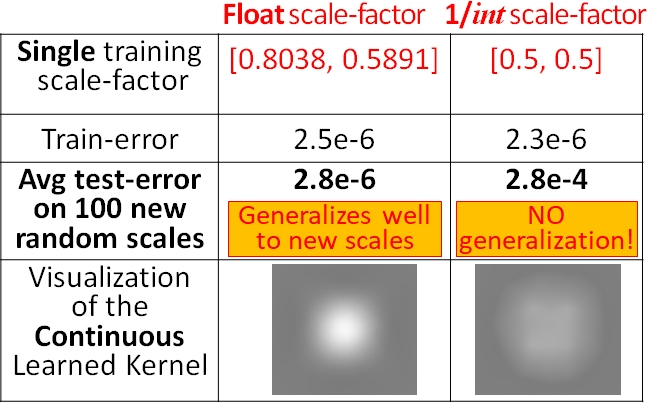
\includegraphics[width=1.1\textwidth]{figs/fig_generalize_Michal.jpg}
   \captionsetup{oneside, margin={-0.1cm,-0.2cm}}
  \captionof{figure}{\it  CC trained on one (float) scale, generalizes well to other scales.}
    \label{fig:generalize}
\end{minipage}

\end{minipage}


\textbf{The power of dynamic Scale-Ensembles at inference:}
%To demonstrate the potential use of CC-layers in image classification tasks, we did the following simple experiment:
Since \michal{the above} ``CC-Net'' was trained with non-integer (float) \michal{internal} scale-factors, it can generalize to new \michal{internal} scale-factors \emph{at inference-time}. This gives rise to \emph{ensemble-based image classification} (Sec.~\ref{sec:features} \& Fig.~\ref{fig:scale_ensemble}). 
This means that our trained CC-Net can be applied numerous times at inference, each time with a different sequence of scales (as long as their product yields 1/4), and average the \niv{logits}
% probabilities
of all forwarded passes.
%We tested this for 1,2,3 applications of CC-Net. Even small ensembles 
\michal{We tested this for CC-Net. Even small ensembles (2,3)}
already gave a significant boost in classification accuracy (+1.7\%, +2.4\%, respectively).
\michal{While test-time augmentations for regular CNNs can be applied  to the input image only, Scale-Ensembles apply test-time augmentation to \emph{all} CC-layers in the network. Hence, deep nets with many CC-layers, are likely to benefit from larger self-ensembles.}
%
% For reference, when providing Baseline-Net with test-time augmentations of the input images (mild scale variations and horizontal-flip) and averaging probabilities, the improvement was very mild 
% %we used mild random scaling (scale-factor between 1 and 1.1) and center-cropping of the input image. We observed that scaling hardly improves their results so we also used horizontal flips for both our test-augmentations and for the baselines.
% Such augmentations gave a slight improvement (up to +1.1\% for 2 augmentations), but not as significant as the scale-ensembles (+2.2\% for 5 ensembles). 

\textbf{Potential use in image-processing tasks:}
CC-layers could potentially be very useful in image-processing tasks. For example, existing Super-Resolution (SR) networks are trained for a fixed scale-factor~\cite{EDSR, srcnn}. To increase the resolution of an image by a factor of 3, one must use a SRx3 net which was trained for this specific scale-factor. SR by a factor of 4 will require a different pretrained SRx4  net. 
Constructing a SR network based on CC-layers is expected to give \emph{SR with any desired scale factor} (or at least an impressive range of scale-factors), all \emph{with a single trained SR net}. 
%Moreover, it should be able to accommodate different SR scale factors for different axes, if so desired.
\michal{Moreover, it could potentially accommodate different SR scale factors for different axes (if so desired). Note that training a separate net for every potential SR scale 
(or any combination of vertical~x~horizontal SR scales) 
is combinatorially daunting. A CC-based SR network may alleviate this problem.}
Designing such a CC-based SR network is part of our future work.

% \section*{Broader Impact}
% This work does not present any foreseeable societal consequence.

% The dynamic features of the new CC-layer has the potential to replace multiple network (for example SR networks for different scales) with a single network, which may yield both better results and may save resources (especially electricity).

\textbf{\it Authors are required to include a statement of the broader impact of their work, including its ethical aspects and future societal consequences. 
Authors should discuss both positive and negative outcomes, if any.} \\

\underline{\textbf{AUTHORS' ANSWER:}}

\textbf{a) Who may benefit from this research?}
Any ML or CV researcher, or code developer, who uses Deep Learning code and designs neural architectures.

\textbf{b) Who may be put at disadvantage from this research?}
No one, to our best knowledge.

\textbf{c) What are the consequences of failure of the system?}
Not applicable. This is not a system, but rather a new useful component in Deep Learning architectures.

\textbf{d) Whether the task/method leverages biases in the data?}
Not to our best knowledge.


\clearpage
\printbibliography

\clearpage
\begin{appendices}
% \renewcommand{\theequation}{\thesection.\arabic{equation}}
% \clearpage
\section{Details of Experiments and Architectures}

\subsection{Internal Net $\mathcal{K}_\theta$}
Table.~\ref{tab:internal} below shows the architecture of the internal net $\mathcal{K}_\theta$ used for all experiments. The properties of each layer is denoted by  \textsc{Conv} $[Channels], [Kernel\_height] \times [Kernel\_width] + [Stride]$. Each Conv layer of  $\mathcal{K}_\theta$ except the last one, is followed by LeakyReLU activation. Each \CC layer contains its own \textsc{InternalNet}$: \mathbb{R}^2 \to \mathbb{R}$ (the learned continuous kernel). The input to \textsc{InternalNet} are distances from a specific pixel position in the output, given as a 4D tensor, and computed using $3$ consecutive 2D 1$\times$1 convolutions, as detailed in the table .

Block 2 in Sec.~\ref{sec:implement_construct} describes the input to $\mathcal{K}_\theta$ -- distances tensor of size $[K,2,H',W']$ where K is the number of neighbors within the support. When applying 2D conv layers to it, the first dimension of the tensor is regarded as the batch dimension. We do so intentionally, as we want to apply the same operation to all neighbor distances in parallel. The final calculated weight tensor is of size $[1,C_{out},C_{in},K,H',W']$, where $C_{in}, C_{out}$ are the numbers of input channels and output channels, respectively. 

By default, the number of channels of the final internal conv layer,  {$C_{final}$} needs to cover both in and out external channels of the CC layer. {$C_{final} = C_{in} \times C_{out}$}, then the calculated weights tensor  can be obtained by simple reshaping of the Internal Net's output: 
$[K, C_{out}\times C_{in}, H', W'] \rightarrow [1,C_{out},C_{in},K,H',W']$. 
In the equivariance experiment we used the efficient implementation mentioned in Sec.~\ref{sec:efficiency}: "No need to keep the Neighbors distances". In this case, the input is just the grid [1,2,H',W'] so the batch size is 1 and {$C_{final} = C_{in} \times C_{out} \times K$} to accommodate for the weights of all the neighbors.

\begin{table}[h!]
    \centering
    \begin{tabular}{lll}
    \toprule
       InternalNet  \\
    \midrule
      \textsc{Conv} 16 1x1+1  \\
      \textsc{Conv} 16 1x1+1  \\
      \textsc{Conv} $C_{final}$ 1x1+1  \\
    \bottomrule
    \end{tabular}
    \vspace{5pt}
    \caption{Architecture used for $\mathcal{K}_\theta$ in all experiments}
    \label{tab:internal}
\end{table}


% \subsection{Shift equivariance experiment -- Classification network architecture}
\subsection{Shift Equivariance Experiments}
All experiments were conducted on \textsc{CIFAR10} dataset \cite{CIFAR10} and implemented using \textsc{PyTorch}~\cite{paszke2017automatic} deep learning framework. 

The architectures we used for the Classification Networks in Sec.~\ref{sec:efficiency} are detailed in Table~\ref{tab:architectures}. \textsc{CC} corresponds to a continuous convolution layer with similar terminology (except that \textsc{CC} layers do not have a fixed stride). \textsc{FC} $n$ corresponds to a fully connected layer with $n$ outputs. Each \textsc{Conv}/\textsc{FC} layer is followed by a ReLU activation except for the last fully connected layer. As can be seen, \textsc{CCNet} and \textsc{ConvNet} share the same general architecture. The models are based on similar models from \cite{wong2018scaling,atzmon2019controlling}, where we added a few more convolution layers to exemplify the gradual change in scale.

\begin{table}[h!]
    \centering
    \begin{tabular}{lll}
    \toprule
         \textsc{ConvNet (Baseline)}  & \textsc{CCNet}\\
    \midrule
         \textsc{Conv} 32 3x3+1     & \CC 32 3x3      \\
         \textsc{Conv} 32 4x4+2     & \CC 32 4x4      \\
         \textsc{Conv} 64 3x3+1     & \CC 64 3x3      \\
         \textsc{Conv} 64 3x3+1     & \CC 64 3x3      \\
         \textsc{Conv} 64 3x3+1     & \CC 64 3x3      \\
         \textsc{Conv} 64 3x3+1     & \CC 64 3x3      \\
         \textsc{Conv} 64 3x3+1     & \CC 64 3x3      \\
         \textsc{Conv} 64 4x4+2     & \CC 64 4x4      \\
         \textsc{FC} 512            & \textsc{FC} 512 \\
         \textsc{FC} 512            & \textsc{FC} 512 \\
         \textsc{FC} 10             & \textsc{FC} 10  \\
    \bottomrule\\
    \end{tabular}
    \vspace{-5pt}
    \caption{Model architectures used for shift-equivariance experiment}
    \label{tab:architectures}
\end{table}


\paragraph{Initialization} The outputs of the \textsc{InternalNet} are equivalent to the weights of an ordinary \textsc{Conv} layer. At initialization, we require those outputs to have a variance similar to an ordinary \textsc{Conv} layer's weights at initialization (either \textit{Xavier} \cite{glorot2010understanding}, \textit{Kaiming} \cite{he2015delving} or the default \textsc{PyTorch}~\cite{paszke2017automatic} initializations). This is done by initializing the biases of the last layer of the \textsc{InternalNet} using a normal distribution with the required variance.

\paragraph{Training Hyperparameters} All models were trained using a batch size of $64$ of images obtained by padding the original CIFAR10 images by 8 rows/cols (4 from each side) and taking a random crop of $32 \times 32$. We also use
% images with random-crops of $32\times 32$ of images padded by 4 rows/cols (2 from each side), 
random horizontal-flip and normalize the inputs to have zero mean and unit variance (as done with common models for training on \textsc{CIFAR10}~\cite{pytorch-cifar}). 
We used \textsc{ADAM} optimizer \cite{kingma2014adam} with weight-decay of $0.0005$. For \textsc{CCNet} we use learning rate of $0.0005$ with a reduction by $10$ on epochs $[200,300]$. For the baseline \textsc{ConvNet} model we checked learning rates $0.0001, 0.0005, 0.001, 0.002$ with several learning rate scheduling (reducing by $10$) at: $[70,150], [150,250], [100,250], [200,300]$, with and without weight-decay, and chose the best performing model of learning rate $0.001$, weight-decay of $0.0005$ and learning rate reduction at epochs $[150,250]$. Results are reported after $400$ epochs, where all our runs seem to fully converge (e.g., further reduction in learning rates did not change the reported results).

\paragraph{Training and Inference with scale-augmentations} 
As mentioned, \CC layers can be given the scale and output shape dynamically during forward pass. In order to train a \textsc{CCNet} model with scale-augmentations we use the following design: the first \CC layer has a fixed scale of $1$ and output shape equal to input shape. We are left with $7$ \CC layers to reduce spatial dimension by $1/4$, that is, we want the product of all $7$ \CC layers' scales to equal to $1/4$. The \CC layers' scales are then sampled from a normal distribution of mean $(1/4)^{(1/7)}$ and standard deviation of $0.01$. All scales are then projected to the nearest rational fraction with a maximal denominator of $10$. At this point we have $7$ scales $\{s_i \}_{i=1}^7$, however $\Pi s_i$ does not necessarily equal to our target scale $1/4$. To this end we uniformly at random choose one layer $j$ and set $s_j = (1/4) / \Pi_{i \neq j} s_i$. At inference time we sample $k$ scales using the same methodology described here. The output shapes are determined by the following:
\begin{equation}
    \mathrm{output\_shape}\left(j\right) = \begin{cases} 
          \Bigl\lceil{\mathrm{input\_shape} \times \Pi_{i=1}^j s_i }\Bigr\rceil & j\mathrm{\ is\ not\ last} \\
          \mathrm{input\_shape} \times (1/4) & j \mathrm{\ is\ last\ layer} \\
   \end{cases}
   \label{eq:output_shape}
\end{equation}

A few examples for scale augmentations are shown in Table~\ref{tab:scale_augs_examples}.

\renewcommand{\arraystretch}{1.3}
\begin{table}[h!]
    \centering
    \begin{tabular}{l|cc|cc}
    \toprule
                & \multicolumn{2}{c}{Augmentation Example 1}                     & \multicolumn{2}{c}{Augmentation Example 2}                        \\
         Layer  &                {Scale [H,W]}                                & $\to$ Output Shape   & {Scale [H,W]} & $\to$ Output Shape         \\
    \midrule
        $1$     &                $[ \frac{1}{1}$    , $\frac{1}{1}]$          &   $[32,32]$          & $[\frac{1}{1}$  , $\frac{1}{1}]$     & $[32,32]$      \\        
        $2$     &                $[ \frac{5}{6}$    , $\frac{7}{9}]$          &   $[27,25]$          & $[\frac{75}{98}$, $\frac{7}{8}]$     & $[25,28]$      \\        
        $3$     &                $[ \frac{5}{6}$    , $\frac{4}{5}]$          &   $[23,20]$          & $[\frac{4}{5}$  , $\frac{2}{3}]$     & $[20,19]$      \\        
        $4$     &                $[ \frac{8}{9}$    , $\frac{5}{6}]$          &   $[20,17]$          & $[\frac{4}{5}$  , $\frac{3}{4}]$     & $[16,14]$      \\        
        $5$     &                $[ \frac{189}{250}$, $\frac{3}{4}]$          &   $[15,13]$          & $[\frac{7}{8}$  , $\frac{5}{6}]$     & $[14,12]$      \\        
        $6$     &                $[ \frac{6}{7}$    , $\frac{6}{7}]$          &   $[13,11]$          & $[\frac{5}{6}$  , $\frac{5}{6}]$     & $[12,10]$      \\        
        $7$     &                $[ \frac{5}{6}$    , $\frac{7}{8}]$          &   $[11,10]$          & $[\frac{7}{9}$  , $\frac{864}{875}]$ & $[9\ ,10]$      \\        
        $8$     &                $[ \frac{3}{4}$    , $\frac{6}{7}]$          &   $[8\ ,\ 8]$        & $[\frac{9}{10}$ , $\frac{5}{6}]$     & $[8\ ,\ 8]$    \\
    \bottomrule
    \end{tabular}
    \vspace{5pt}
    \caption{Examples of scale augmentations. $[H,W]$ corresponds to each spatial dimension. The model consists of $8$ continuous convolution layers (where the first is fixed to a scale $[1,1]$), input-shape is $[32,32]$ and target-scale is $[\nicefrac{1}{4},\nicefrac{1}{4}]$. The output shapes are computed from the scales and input shape using Equation~\ref{eq:output_shape}.}
    \label{tab:scale_augs_examples}
\end{table}

% \begin{figure}[h!]
%     \centering
%     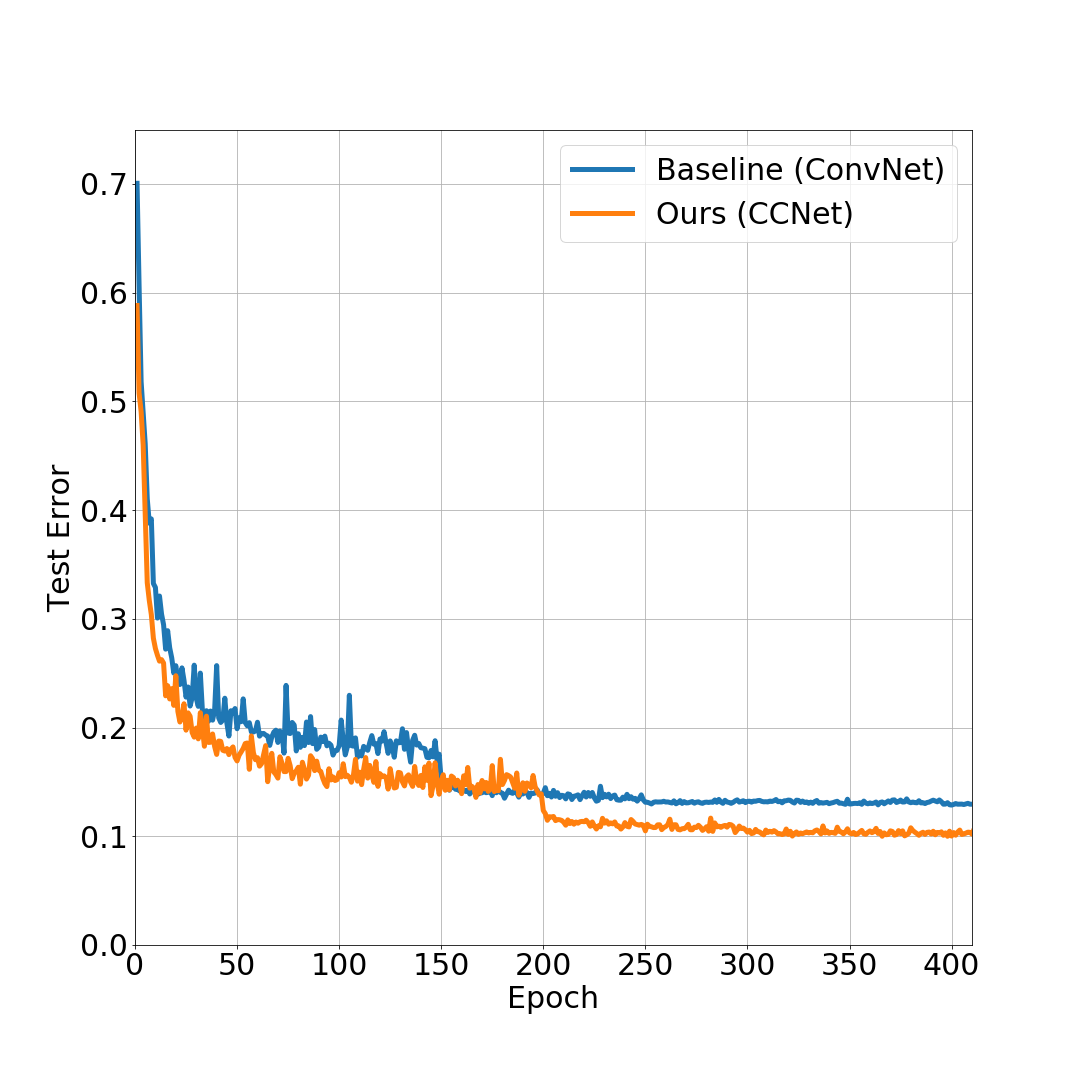
\includegraphics[width=0.65\columnwidth]{figs/classification_error.png}
%     \caption{Test error per epoch of our trained models}
%     \label{fig:training}
% \end{figure}

% \clearpage
\section{Runtime and Memory Analysis}
\subsection{CC Layers}
We measured the runtime and memory consumption of CC layers, with varying input size and number of consecutive layers. We show that our efficient implementation techniques (introduced in Sec.~\ref{sec:efficiency}) significantly reduce the memory footprint of a CC-layer, and some techniques (implementation using discrete convolutions) further speed up the layer. For reference, we also compare to a Conv-layer, although it lacks the expressiveness of the CC-layer. In the column ``CC (clear memory)'' (see Tables~\ref{tab:runtime_by_sz} and~\ref{tab:runtime_by_num_layers}), we divided the computation into chunks of size $32\times32$, computed the results sequentially and discarded all intermediate results (see "Saving memory by keeping only $\mathcal{K}_\theta$" in Sec.~\ref{sec:efficiency}). This implementation supports non-rational scales, and allows us to use deeper networks than the non-optimized implementation (``CC (standard)'' column). In the column ``CC (by discrete conv)'', the number of computed filters is reduced from the output size to the numerator of the scale factor -- in our case the scale factor is $\nicefrac{2}{3}$ so we have 2 filters. This mechanism is further optimized by using the convolution operation as backend (see "Efficient implementation using discrete convolutions" in Sec.~\ref{sec:efficiency}). This implementation significantly reduces memory consumption and runtime, at the cost of expressiveness -- as it only supports rational scale factors (and is beneficial as long as the numerator is small).

In terms of runtime, we measured the time of a single forward and backward pass through the layer (or layers). To accurately measure the time, we run 11 repeats and excluded the first (warm-up), and report the average of the last 10 (the deviation was negligible). In terms of memory consumption, we report the peak allocated memory in GiB ($2^{30}$ bytes). Sometimes there is a difference between the peak reserved memory and the peak allocated memory, but that's more related to the internals of \textsc{PyTorch}~\cite{paszke2017automatic}. All the tests were conducted on a single Tesla V100-PCIE-16GB GPU.

Table.~\ref{tab:runtime_by_sz} shows the runtime and memory consumption of a single layer with varying input size. In all the experiments we used a $3\times3$ kernel with 32 input channels and 32 output channels, and a batch size of 50. For the CC-layer, we used inner architecture as in Table.~\ref{tab:internal} with scale of $\nicefrac{2}{3}$. For the Conv-layer, we used stride of 1.

Table.~\ref{tab:runtime_by_num_layers} shows the runtime and memory consumption of multiple layers with a fixed input size of $64\times64$. In this experiment we used the same parameters, except for the scale -- here we used a scale of $1$ to have the same input size in all layers.

\begin{table}[h!]
    \centering
    \begin{tabular}{c|cccc}
    \toprule

Input Size     & CC (standard)     & CC (clear memory) & CC (by discrete convs) & Conv (reference) \\
\midrule
$32\times32$   & 8.7ms / 0.9GiB    & 19.7ms / 1.8GiB   & 3.5ms / 0.1GiB         & 0.8ms / 0.1GiB   \\
$64\times64$   & 30.0ms / 3.4GiB   & 76.1ms / 3.7GiB   & 3.6ms / 0.2GiB         & 1.3ms / 0.2GiB   \\
$96\times96$   & 72.3ms / 7.6GiB   & 155.4ms / 3.9GiB  & 5.1ms / 0.4GiB         & 2.7ms / 0.5GiB   \\
$128\times128$ & 131.5ms / 13.6GiB & 285.9ms / 4.1GiB  & 7.6ms / 0.7GiB         & 4.0ms / 0.4GiB   \\
    \bottomrule

    \end{tabular}
    \vspace{5pt}
    \caption{Runtime and memory consumption of CC-layer with varying input size.}
    \label{tab:runtime_by_sz}
\end{table}

\begin{table}[h!]
    \centering
    \begin{tabular}{c|cccc}
    \toprule
\# Layers & CC (standard)   & CC (clear memory) & CC (by discrete convs) & Conv (reference) \\
\midrule
1        & 71.7ms / 7.5GiB & 158.7ms / 3.8GiB  & 3.5ms / 0.3GiB         & 1.3ms / 0.2GiB   \\
2        & OUT OF MEMORY   & 317.9ms / 3.9GiB  & 7.0ms / 0.3GiB         & 2.8ms / 0.3GiB   \\
4        & OUT OF MEMORY   & 635.0ms / 4.0GiB  & 14.1ms / 0.4GiB        & 6.0ms / 0.4GiB   \\
8        & OUT OF MEMORY   & 1270.2ms / 4.2GiB & 27.1ms / 0.7GiB        & 12.5ms / 0.6GiB  \\
16       & OUT OF MEMORY   & 2538.7ms / 4.6GiB & 54.6ms / 1.1GiB        & 25.2ms / 1.0GiB  \\
32       & OUT OF MEMORY   & 5074.7ms / 5.5GiB & 111.3ms / 2.0GiB       & 51.6ms / 1.8GiB  \\
    \bottomrule
    \end{tabular}
    \vspace{5pt}
    \caption{Runtime and memory consumption of varying number of consecutive CC-layers.}
    \label{tab:runtime_by_num_layers}
\end{table}

\subsection{CC Classification Networks}
\textsc{Baseline ConvNet} takes 6 seconds per epoch, while \textsc{CCNet} takes 90 seconds per epoch. This difference is mainly attributed to the fact that CC-layer has a constant overhead of computing the weights, which is independent of the spatial size (when using conv implementation) and thus more significant when the input is small. Also, the feature maps in the \textsc{CCNet} are always (spatially) larger than in \textsc{Baseline ConvNet} due to the gradual downscaling. Finally, some scale factors (which were randomly chosen at each iteration) has large numerator which reduces the speed of the conv-based implementation.

\end{appendices}


\end{document}
